\chapter{Diseño e Implementación} % Main chapter title

\label{Chapter3} % Change X to a consecutive number; for referencing this chapter elsewhere, use \ref{ChapterX}
\definecolor{mygreen}{rgb}{0,0.6,0}
\definecolor{mygray}{rgb}{0.5,0.5,0.5}
\definecolor{mymauve}{rgb}{0.58,0,0.82}

%----------------------------------------------------------------------------------------

En este capítulo se explican los criterios utilizados en el desarrollo del prototipo y se justifican las decisiones de diseño; así como también se describe la implementación.

\section{Hardware}
\label{section:hardware}

En el contexto del presente trabajo, se desarrolló un prototipo funcional del producto final. Este prototipo presenta las mismas funciones que el equipo final pero no se ajusta a los lineamientos estéticos y mecánicos que si deberá cumplir en un futuro. Es por esto que el prototipo diseñado tiene dimensiones mucho más grandes que las que tendrá, lo cual facilitó las mediciones y pruebas que se debieron realizar para comprobar el correcto funcionamiento tanto del hardware como del firmware. 

En la Figura \ref{fig:prototipo} puede verse una fotografía del prototipo. En la misma se puede apreciar el PCB diseñado y las dos conexiones principales: a la izquierda del gabinete la conexión a la línea eléctrica y a la derecha la conexión a la carga eléctrica. La placa fue colocada dentro de un gabinete que no tiene relación alguna con el gabinete que finalmente se utilizará. Simplemente cumple la función de facilitar la manipulación del prototipo.

\begin{figure}[h]
	\centering
	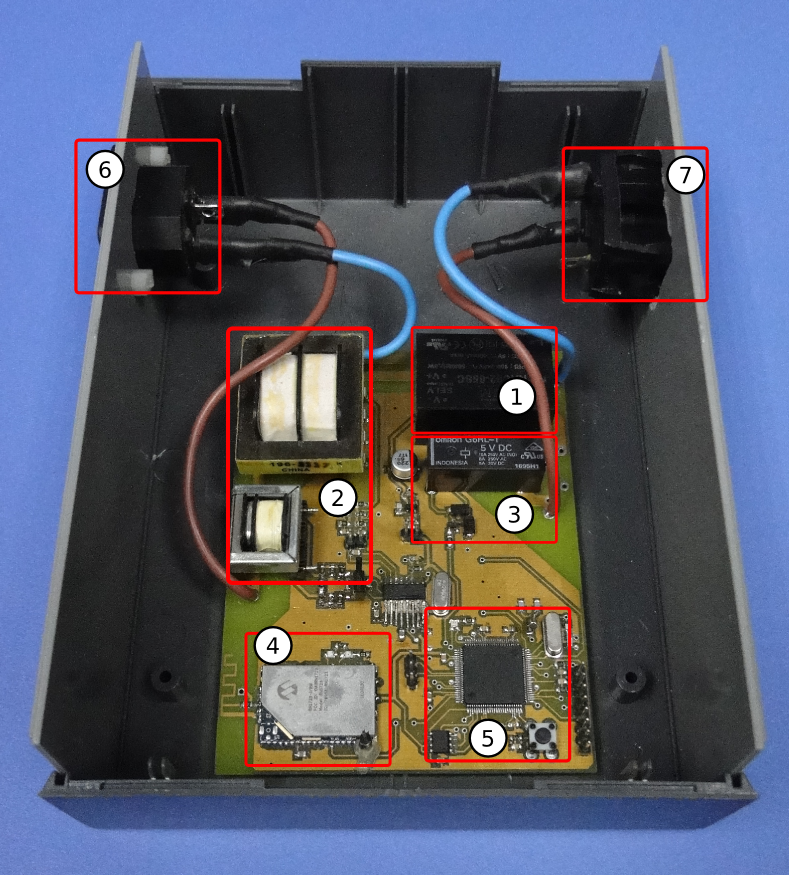
\includegraphics[width=11cm]{./Figures/3_1_prototipo_1.png}
	\caption{Prototipo funcional del Smart Plug. 1 - Fuente de alimentación. 2 - Adaptación de las señales de línea. 3 - Control de la carga. 4 - Módulo WiFi. 5 - Microcontrolador, led bicolor, pulsador y memoria EEPROM. 6 - Conexión a la línea eléctrica. 7 - Conexión a la carga.}
	\label{fig:prototipo}
\end{figure}

Los bloques mencionados en la Figura \ref{fig:prototipo} son explicados en las Subsecciones \ref{subsec:esquematico_general} y \ref{subsec:detalles_hardware}.

A pesar de ser un prototipo funcional, el hardware se diseño pensando en las características finales que tendrá el producto. Por lo tanto se debieron definir las especificaciones deseadas para el equipo:

\begin{itemize}
\item Tensión máxima de operación: 240VAC
\item Corriente máxima de operación: 5A
\end{itemize}

Para una tensión de operación de 220VAC, la máxima potencia que se puede conectar es de 1100W. Para un primer producto se buscó cubrir la automatización de aparatos eléctricos de baja potencia como lámparas, ventiladores, electrodomésticos pequeños, televisores, etc. El manejo de equipos de mayor potencia como aires acondicionados, estufas eléctricas, hornos eléctricos, etc, será cubierto en un futuro cuando se modifique el hardware para soportar una mayor corriente, generando así un nuevo producto.



\subsection{Esquemático general}
\label{subsec:esquematico_general}

En la Figura \ref{fig:hardware_diagrama_bloques} pueden verse los principales bloques funcionales del prototipo.

\begin{figure}[h]
	\centering
	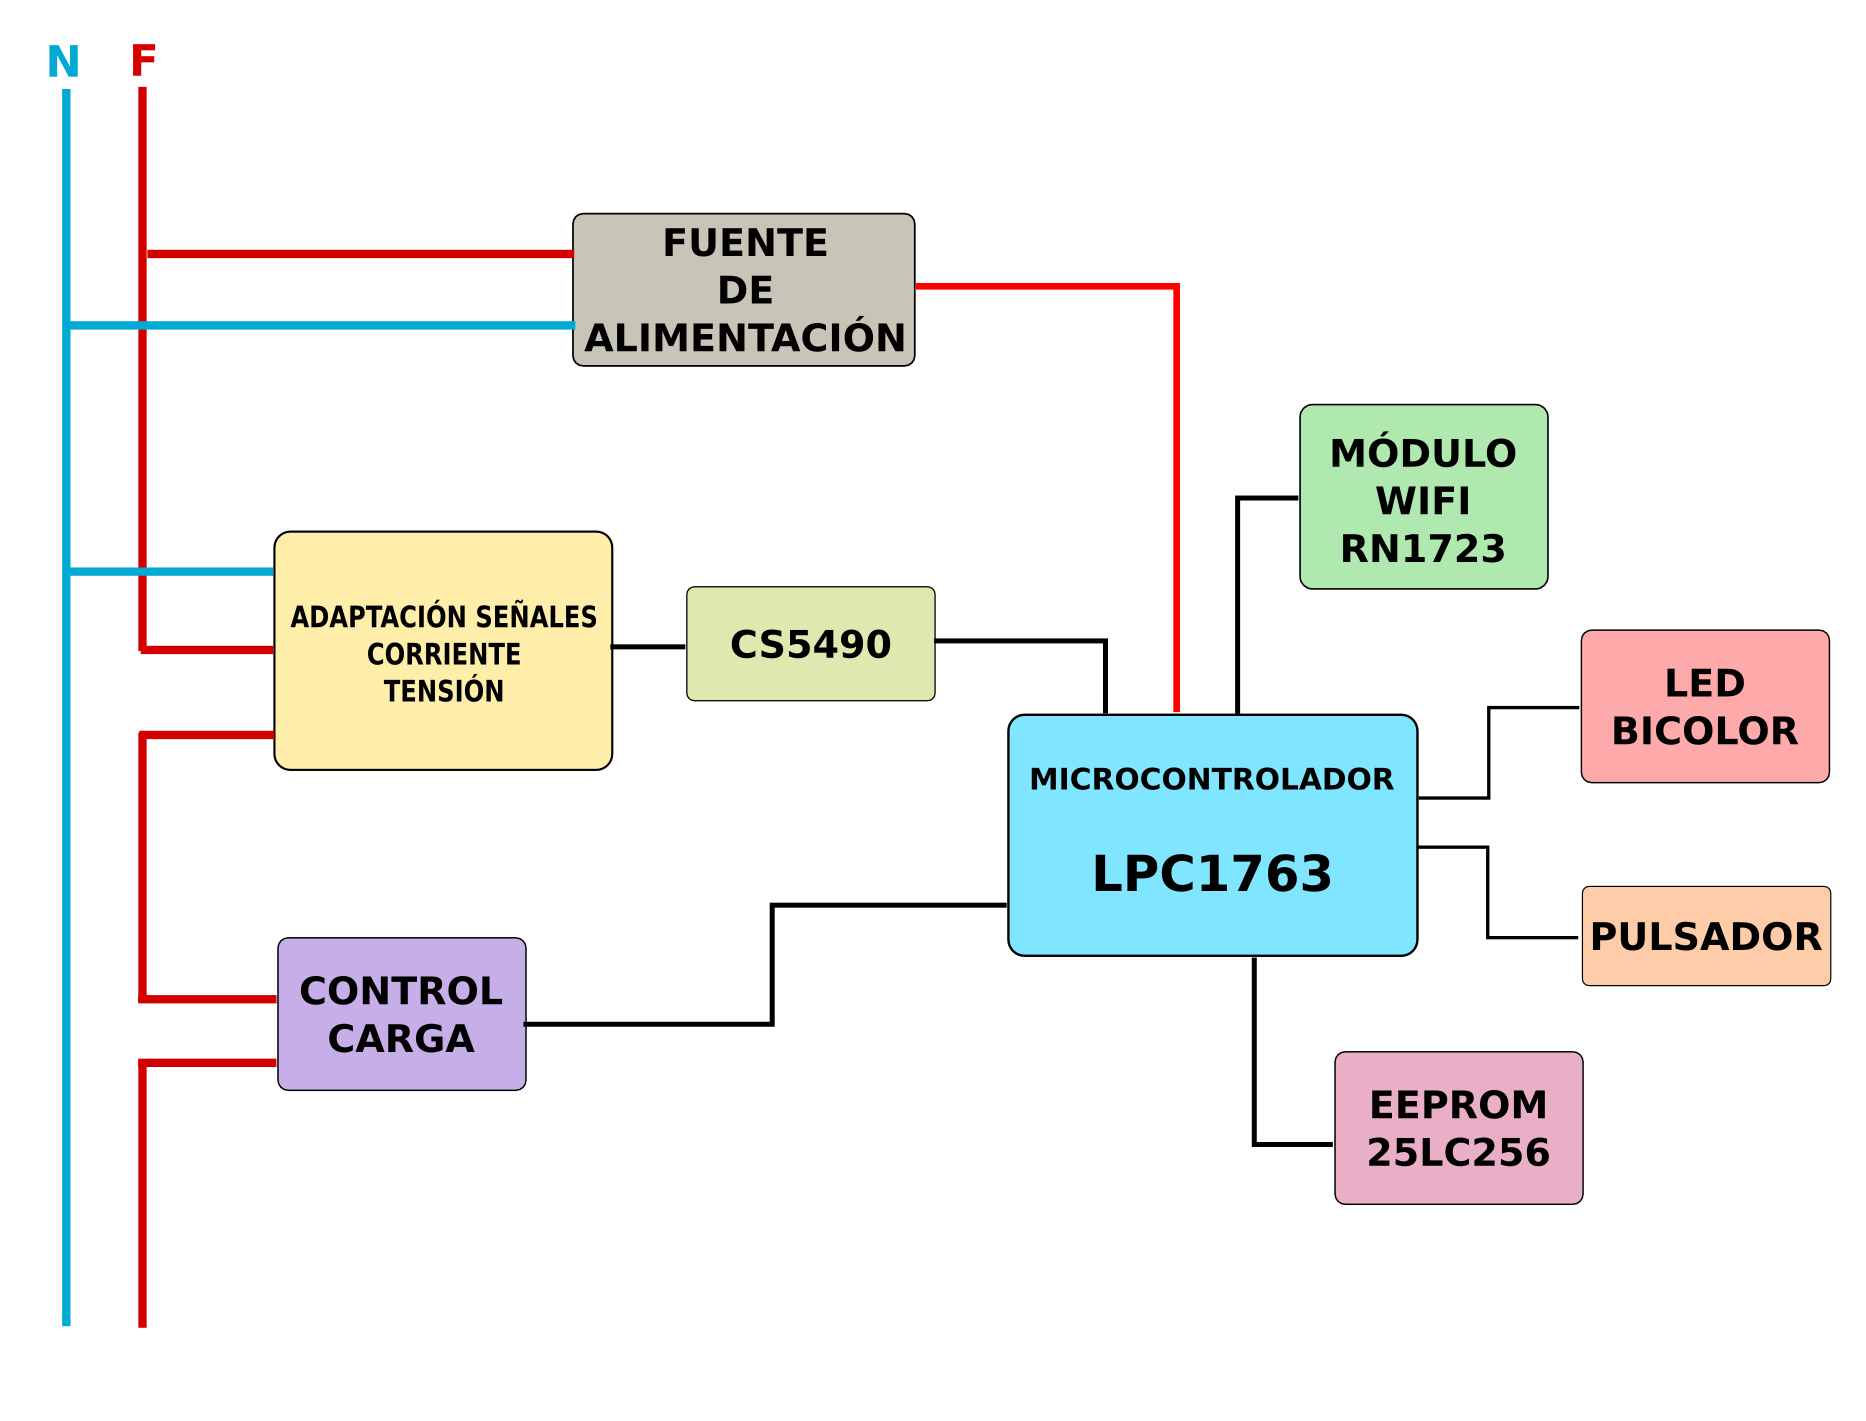
\includegraphics[width=12cm]{./Figures/3_1_1_diagrama_bloques_hardware.png}
	\caption{Diagrama en bloques del hardware del prototipo funcional.}
	\label{fig:hardware_diagrama_bloques}
\end{figure}

A continuación se describe brévemente cada uno de los módulos. Una explicación más detallada de cada uno se encuentra en la Subsección \ref{subsec:detalles_hardware}:

\begin{itemize}
\item Fuente de alimentación. La alimentación del equipo es obtenida de la misma línea eléctrica a la que está conectado el dispositivo. Debe generar dos niveles de tensión, 5V y 3,3V y debe ser capaz de soportar el consumo especialmente del módulo WiFi.
\item Adaptación de las señales de corriente y tensión. Este bloque se encarga de adaptar la señal de tensión de la línea y la señal de la corriente consumida por el aparato eléctrico a los niveles que requiere el front-end analógico CS5490. La adaptación se realiza mediante transformadores para lograr una completa aislación de la línea.
\item Front-end analógico CS5490. Es el circuito integrado encargado de tomar las señales de la línea y generar las mediciones eléctricas de interés: tensión eficaz, corriente eficaz, frecuencia de línea, factor de potencia, energía consumida, etc.
\item Control de la carga. La conmutación de la carga se realiza mediante un relay mecánico.
\item Módulo WiFi RN1723. Es el módulo encargado de la comunicación entre el Smart Plug y la aplicación móvil. Básicamente se encarga de esperar conexiones TCP y enviar las respuestas requeridas al socket del que provino el comando.
\item Microcontrolador LPC1763. Es el encargado de implementar la lógica del Smart Plug. 
\item Memoria EEPROM. Es la encargada de retener información de configuración del Smart Plug y las mediciones diarias de potencia y energía.
\item Led bicolor. Es un led rojo y verde encargado de realizar las señalizaciones acerca del funcionamiento del equipo. En la Subsección \ref{subsec:firmware_arquitectura} se describe el significado de las distintas señalizaciones.
\item Pulsador. Mediante el pulsador se inician los procesos destinados a incorporar el Smart Plug a la red WiFi de la casa.
\end{itemize}

\subsection{Descripción de los módulos de hardware}
\label{subsec:detalles_hardware}

En este apartado de la memoria se describen las decisiones de diseño asociadas a los módulos de hardware. Los fragmentos de esquemático que a continuación se muestran surgen del archivo \textit{SmartPlug\_v1.0} en \citep{repo_hardware}.

\subsubsection{Fuente de alimentación}

El esquemático de la fuente del Smart Plug puede verse en la Figura \ref{fig:pcb_fuente}. Esta fuente de alimentación se conecta a la misma línea eléctrica que es medida por el front-end analógico. A partir de la tensión de 220VAC genera una tensión de 5V y 3,3V. Para lograr los 5V se utiliza una fuente switching con montaje para PCB VSK-S2-5U la cual puede entregar hasta 400mA. Esta fuente permite generar una tensión estable manteniendo un empaquetado de reducido tamaño (34 x 22 x 18 mm). 

\begin{figure}[h]
	\centering
	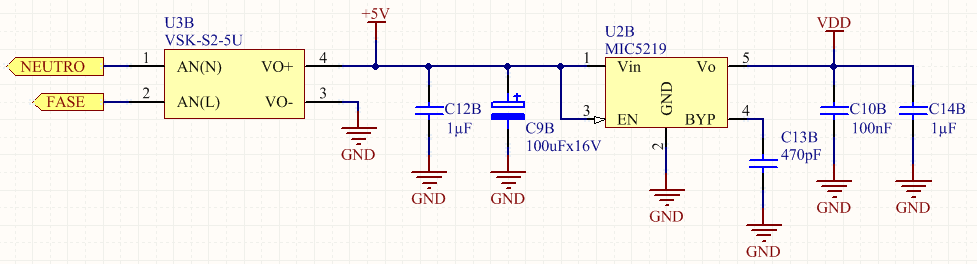
\includegraphics[width=14cm]{./Figures/3_1_2_pcb_fuente.png}
	\caption{Esquemático de la fuente de alimentación.}
	\label{fig:pcb_fuente}
\end{figure}


Se debe aclarar que esta fuente switching fue elegida para el prototipo funcional. En la versión final del equipo se utilizará una fuente switching AC-DC de similares características diseñada dentro de la empresa X-28 Alarmas, debido a que tanto el tamaño del empaquetado de la fuente como su costo (U\$s 13,25 por unidad al momento de escribir la memoria) son prohibitivos para incluir esta fuente en el diseño final.

En cuanto al regulador de 3,3V se eligió un componente que puede entregar hasta 500mA. El requerimiento de corriente tanto de la fuente switching como del regulador de 3,3V surge del consumo especialmente del módulo WiFi RN1723, el cual puede requerir hasta 250mA.


\subsubsection{Adaptación de las señales de tensión y corriente}

En la Figura \ref{fig:pcb_adaptacion} puede verse la sección del esquemático relacionada con la adaptación de las señales de tensión y de corriente del dispositivo. Para poder obtener las mediciones eléctricas y el consumo de la carga conectada al Smart Plug es necesario adaptar las señales de tensión de línea y de la corriente consumida por la carga a los niveles soportados por el front-end analógico.

\begin{figure}[h]
	\centering
	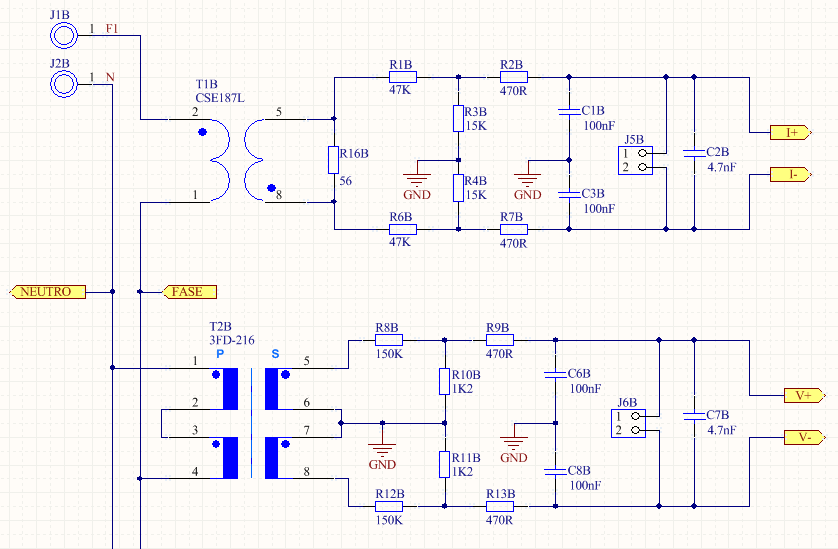
\includegraphics[width=14cm]{./Figures/3_1_2_pcb_adaptacion.png}
	\caption{Esquemático de la etapa de adaptación de las señales de tensión y corriente de la línea eléctrica.}
	\label{fig:pcb_adaptacion}
\end{figure}

De acuerdo a la hoja de datos del front-end elegido para este proyecto (CS5490) tanto la señal de corriente como la de tensión no deben superar los 250mV de pico en las entradas diferenciales del circuito integrado. Para lograr esto, primero se debe definir la tensión y la corriente máxima que debe medir el Smart Plug. En el caso concreto de este proyecto, y como ya fue mencionado, estos valores son: tensión máxima - 240VAC, corriente máxima - 5A.

Definidos estos valores, se eligió aislar el resto del circuito de la línea eléctrica tomando las señales de tensión y corriente mediante transformadores. Al igual que sucedió con la elección de la fuente switching, esta decisión fue exclusivamente para el desarrollo del prototipo funcional, ya que en la versión final será conveniente reemplazar el transformador de tensión por divisores resistivos y el transformador de corriente por un shunt. Ambos cambios van a permitir reducir el tamaño del producto final y su costo.

Luego de los transformadores hay divisores resistivos dispuestos en forma diferencial para reducir la tensión a los valores tolerados por el CS5409. Finalmente hay filtros pasa-bajo con un a frecuencia de corte de 3,3kHz.

Con los valores elegidos de relación de transformación y divisores resistivos, los valores máximos soportados por el equipo resultan:

\begin{itemize}
\item Tensión máxima soportada por el hardware: 320VAC.
\item Corriente máxima soportada por el hardware: 6,5A.
\end{itemize}

Ambos valores se encuentran por encima de los valores máximos informados al usuario.


\subsubsection{Front-end analógico}

Luego de adaptar las señales de tensión y de corriente, las mismas deben ser medidas por un front-end analógico que se encargará de generar los parámetros de interés para la aplicación: tensión y corriente eficaz, frecuencia de línea, potencia activa, factor de potencia, energía consumida, etc. En la Figura \ref{fig:pcb_medicion_energia} puede verse el circuito asociado al front-end elegido, el CS5490.

\begin{figure}[h]
	\centering
	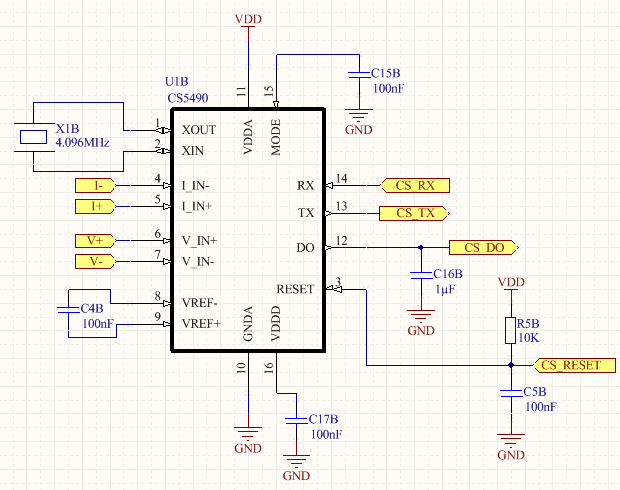
\includegraphics[width=14cm]{./Figures/3_1_2_pcb_medicion_energia.png}
	\caption{Esquemático del front-end analógico encargado de medir los parámetros eléctricos.}
	\label{fig:pcb_medicion_energia}
\end{figure}

A parte de los componentes relacionados con la adaptación de las señales de línea, este circuito integrado  no necesita de una gran cantidad de componentes adicionales, salvo algunos capacitores y un cristal de 4,096Mhz con el cual va generar la base de tiempo interna para realizar las mediciones y cálculos.

La comunicación es sencilla, a través de comandos enviados por una UART. Con estos comandos se van poder conocer casi todas las mediciones que calcula el CS5490. La única medición que no puede ser conocida a través de la lectura de un registro es la energía consumida. Esta es informada mediante pulsos a través del pin \textit{DO}. Para esto se debe configurar la constante del medidor en el CS5490, es decir la cantidad de pulsos a los que equivale un kilowatt-hora.


\subsubsection{Control de la carga}

La conmutación de la carga está a cargo de un relay mecánico. En la Figura \ref{fig:pcb_control_carga} puede verse que la fase de la línea eléctrica se conecta entre los contactos \textit{común} y \textit{normal cerrado} del relay para que, en caso de ocurrir un desperfecto con el Smart Plug, la carga pueda seguir funcionando.

\begin{figure}[h]
	\centering
	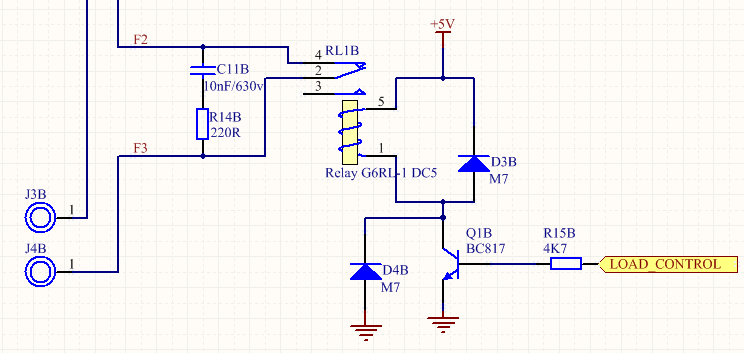
\includegraphics[width=10cm]{./Figures/3_1_2_pcb_control_carga.png}
	\caption{Esquemático del control de la carga eléctrica mediante un relay mecánico.}
	\label{fig:pcb_control_carga}
\end{figure}

Para funcionar, la bobina del relay requiere de una tensión de 5V y los contactos soportan una corriente máxima de 8A con 250VAC, valor que satisface sobradamente las especificaciones propuestas para el Smart Plug.

\subsubsection{Módulo WiFi}

El módulo elegido es el RN1723, el cual prácticamente no requiere de componentes adicionales y se comunica con el microcontrolador mediante una UART.

Para la antena del módulo se eligió una antena impresa en el PCB de acuerdo a las especificaciones de la hoja de datos del módulo.

Al momento de comenzar con el proyecto y elegir los componentes, este módulo resultaba una opción atractiva, que proveía las funcionalidades especificadas en los requerimientos del producto a un precio aceptable. Además se decidió elegir este módulo ya que es comercializado por Microchip, marca que es ampliamente usada por los productos de X-28 Alarmas, lo cual lleva a la posibilidad de obtener precios muy competitivos con los distribuidores.

\section{Firmware}

\subsection{Arquitectura del firmware}
\label{subsec:firmware_arquitectura}

El firmware embebido en el Smart Plug se escribió utilizando FreeOSEK como sistema operativo de tiempo real. De esta forma, en la Figura \ref{fig:firmware_esquema_tareas} pueden verse las tareas que se crearon y la interacción que hay entre estas.

Básicamente, las características del firmware surgen de los requerimientos enumerados en la Sección \ref{sec:requerimientos} y son:

\begin{itemize}
\item Iniciar el proceso de WPS o configurarse en modo punto de acceso (AP) cuando se presiona el pulsador presente en la placa.
\item Mostrar el estado del dispositivo a través del led bicolor.
\item Escuchar las conexiones TCP que provengan de las aplicaciones móviles y generar las respuestas adecuadas.
\item Guardar de forma no volátil (en la memoria EEPROM) la potencia activa promedio y energía consumida de cada hora del día. En la EEPROM se guarda la información de los últimos 7 días.
\item  Sincronizar la hora del Smart Plug con un servidor NTP y gestionar el encendido y apagado de la carga de acuerdo a la programación horaria configurada.
\end{itemize}

\begin{figure}[h]
	\centering
	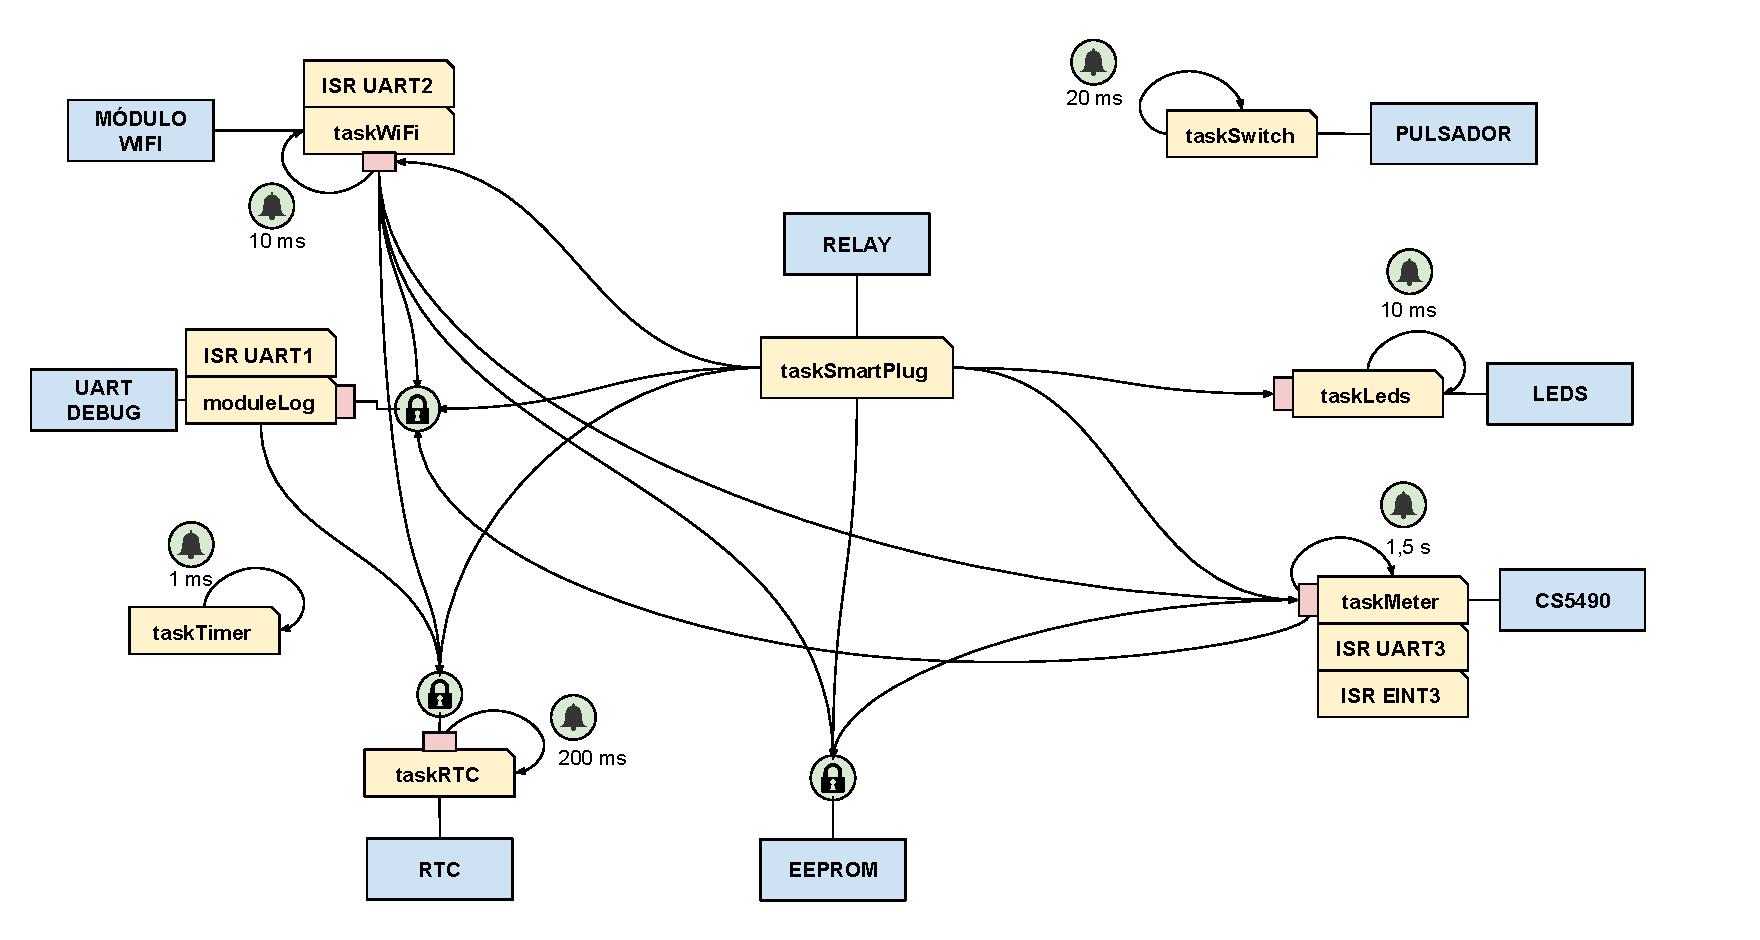
\includegraphics[width=14cm]{./Figures/3_2_1_firmware_esquema_tareas.pdf}
	\caption{Esquema de las tareas y recursos utilizados en el firmware.}
	\label{fig:firmware_esquema_tareas}
\end{figure}

A continuación se describe cada una de las tareas:

\begin{itemize}
\item taskSmartPlug. Es la tarea principal del Smart Plug. Implementa la lógica del dispositivo. Se encarga de recibir los eventos generados por el resto de las tareas y realizar acciones en base a los mismos. Se bloquea esperando que ocurra alguno de los eventos. 

De taskWiFi obtiene los eventos relacionados con la conexión a la red WiFi y las conexiones TCP. Además le indica cuando tiene que iniciar un proceso de WPS o configurarse como punto de acceso.

A taskLeds le indica la señalización que debe realizar de acuerdo al evento recibido. En la Tabla \ref{tab:senializacion_leds} puede verse un resumen de todas las posibles señalizaciones.

De taskMeter obtiene las últimas mediciones para guardarlas de forma no volátil en la memoria EEPROM e ir generando un registro de potencia activa y energía consumida por hora de los últimos 7 días.

Además se encarga de manejar el relay que conmuta la carga eléctrica. El encendido o apagado de la misma se va a determinar a partir de la programación horaria (si está configurada) y de los comandos de encendido y apagado que envíe la aplicación móvil.

\item taskSwitch. Gestiona el pulsador de tipo tact switch que se encuentra en el PCB. Realiza el anti-rebote y genera los eventos cuando es presionado. Va a generar un evento cuando se suelte el pulsador (lo cual inicia el proceso de WPS en el módulo WiFi) y otro cuando se mantenga presionado por más de 5 segundos (lo cual configura al módulo WiFi como un punto de acceso). 

Es una tarea que se ejecuta cada 20ms mediante una alarma de FreeOSEK.


\item taskLeds. Se encarga de realizar las señalizaciones indicadas por otras tareas. Las señalizaciones se forman a partir de un led bicolor (rojo y verde), tanto encendiéndolos, apagándolos o haciéndolos destellar a distintas frecuencias.
Es una tarea periódica que se ejecuta cada 10ms, mediante una alarma de FreeOSEK, para actualizar los leds.


\item taskRTC. Se encarga de configurar y acceder al RTC interno del microcontrolador. Es la tarea que genera los eventos para indicar el paso de un minuto, una hora o un día, los cuales son utilizados por taskSmartPlug para registrar las mediciones de potencia activa y energía consumida por hora.

\item taskWiFi. Se encarga de recibir las conexiones desde la aplicación móvil. Interacciona con taskMeter para requerir las últimas mediciones de acuerdo a lo solicitado por la aplicación móvil.

También consulta la memoria EEPROM para leer o modificar los parámetros de configuración del Smart Plug y para enviarle a la aplicación móvil las mediciones históricas de potencia activa y energía consumida.

Cuando se inicia la tarea, se conecta con un servidor NTP para obtener la fecha y hora. Estos parámetros son enviados a la tarea taskRTC para que configure el RTC interno del microcontrolador.

La comunicación con el módulo es a través de una UART y tanto la recepción como la transmisión se realizan a través de la interrupción de este periférico. La tarea es periódica, cada 10ms, para procesar los mensajes que llegan desde el módulo RN1723  de forma asincrónica.

\item taskMeter. Se encarga de obtener periódicamente las mediciones del front-end analógico CS5490. Además acumula los pulsos generados por el mismo integrado para llevar un registro de la energía consumida por la carga.

Al iniciar la tarea, se encarga de configurar el CS5490 para que funcione de acuerdo a lo especificado. Este proceso incluye:

\begin{itemize}
\item Configurar la constante del medidor. Es la cantidad de pulsos a los que equivale un kilowatt-hora. Para este proyecto se eligió una constante de 5000 pulsos/kWh. Esta constante no es configurada directamente en el CS5490, sino que se deben escribir algunos registros del integrado para lograr que genere 5000 pulsos por kWh. El proceso para lograr esto se explica en la Sección 5.5 de \citep{datasheet_CS5490}.
\item Configurar la tensión y corriente máxima de operación, ya que algunas mediciones van a ser calculadas a partir de estos parámetros.
\item Cargar los valores de calibración. Para lograr los valores de error relativo en el canal de tensión y de corriente que informa la hoja de datos es necesario realizar un proceso de calibración del equipo. Básicamente este proceso consta de dos etapas: calibración de \textit{offset} de continua y calibración de ganancia. Para el primero se deben cortocircuitar las entradas diferenciales del canal de tensión y de corriente y comenzar el proceso. Para la calibración de ganancia, en el caso de la tensión, se debe generar la tensión máxima que puede medir el Smart Plug y comenzar el proceso de calibración. Para el caso de la corriente, se puede usar una corriente menor a la máxima del Smar Plug que debe ser indicada al CS5490 antes de comenzar con la calibración.
Este proceso se encuentra detalladamente explicado en la Sección 7.1 de \citep{datasheet_CS5490}.

En el contexto del presente trabajo el proceso de calibración no se incluyó. Los valores de calibración se calcularon y luego se ajustaron manualmente para cada equipo. En la Sección \ref{sec:trabajo_futuro} se propondrá una posible forma de implementar la etapa de calibración en el proceso de fabricación del producto final.
\end{itemize}

La comunicación con el CS5490 se realiza a través de una UART y tanto la recepción como la transmisión se realizan a través de la interrupción de este periférico. Además se utiliza otra interrupción, encargada de detectar los pulsos generados por el CS5490 para indicar la energía consumida.

Es una tarea periódica que se ejecuta cada 1,5 segundos mediante una alarma de FreeOSEK.

\item moduleLog. Es la tarea encargada de enviar información de la actividad de la aplicación a través de mensajes por una UART. Otras tareas le envían mensajes que debe sacar por la UART, incluyendo la fecha y la hora en la que se produjo el mensaje. Esto tuvo una especial importancia al momento de desarrollar el firmware para conocer los eventos que se estaban produciendo. Los mensajes son enviados a una velocidad de 115200 baudios y se debe conectar un adaptador TTL-USB en la tira de pines destina a la UART en el PCB (llamada DEBUG en el esquemático).

\end{itemize}


\begin{table}[h]
	\centering
	\caption[Señalizaciones del Smart Plug]{Señalizaciones del Smart Plug a través del led bicolor.}
	\begin{tabular}{c c c c c}    
		\toprule
		\textbf{Señalización} 	 & \textbf{Modo AP}  & \textbf{Modo WPS}  & \textbf{Autenticado}  & \textbf{RTC Sincronizado} \\
		\midrule
		Verde destella a 2Hz	 	& 1  & X  & X  & X \\		
		Verde destella a 1Hz	 	& 0  & 1  & X  & X \\
		Rojo destella a 1Hz	 		& 0  & 0  & 0  & X \\
		Verde y rojo destellan	 	& 0  & 0  & 1  & 0 \\
		Verde encendido	 			& 0  & 0  & 1  & 1 \\
		\bottomrule
		\hline
	\end{tabular}
	\label{tab:senializacion_leds}
\end{table}


\subsection{Capas de abstracción}

Para lograr una mayor abstracción del hardware, se decidió implementar el firmware dividiéndolo en capas como se muestra en la Figura \ref{fig:firmware_diagrama_capas}.

\begin{figure}[h]
	\centering
	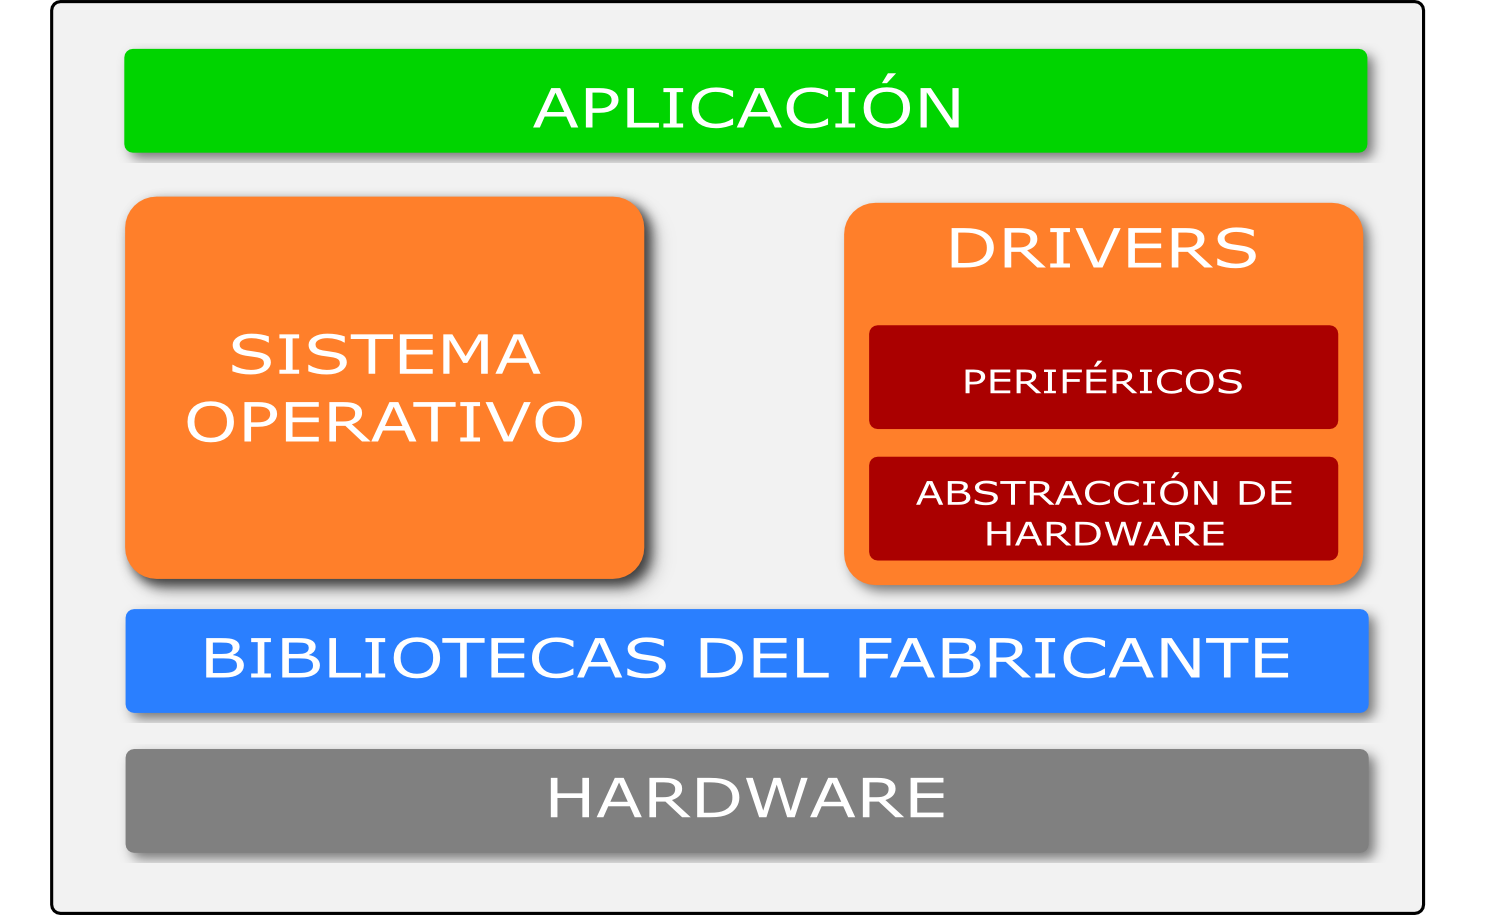
\includegraphics[width=10cm]{./Figures/3_2_2_firmware_diagrama_capas.png}
	\caption{Capas del firmware.}
	\label{fig:firmware_diagrama_capas}
\end{figure}

A continuación se realiza una breve descripción de cada una de las capas:

\begin{itemize}
\item Aplicación. Consiste en el firmware propio del equipo, que utiliza al sistema operativo para implementar la lógica del Smart Plug.
\item Sistema operativo. Consiste en las librerías de FreeOSEK. Como se utilizó un microcontrolador LPC1763 se utilizó la implementación de FreeOSEK para el LPC1769 realizada por Pablo Ridolfi en \citep{repo_ridolfi_freeosek}.
\item Drivers. Dentro de los drivers se encuentran las bibliotecas particulares para controlar tanto los periféricos internos del microcontrolador como los dispositivos externos. La capa de abstracción de hardware, también conocida como HAL (por sus siglas en inglés, Hardware Abstraction Layer), busca generar un nivel más de abstracción entre los drivers de alto nivel y las bibliotecas del fabricante del microcontrolador, lo cual permite, que ante un cambio en el microcontrolador, solamente se deba cambiar la capa HAL.

Para implementar los controladores se utilizó un enfoque orientado a objetos para ordenar las distintas "clases". Una explicación detallada de este proceso se encuentra en la Subsección \ref{subsec:orientado_a_objetos}.
\item Bibliotecas del fabricante. Son las bibliotecas provistas por NXP para acceder a los periféricos internos del microcontrolador.
\item Hardware. Componentes del Smart Plug.
\end{itemize}

\subsection{Metodología orientada a objetos}
\label{subsec:orientado_a_objetos}

Para implementar los drivers, tanto de los periféricos internos del microcontrolador como de los módulos externos, se decidió utilizar una metodología orientada a objetos, a pesar de estar programando en C. La forma de estructurar el código surgió a partir de lo explicado por Alex Schreiner en su libro \textit{Object-Oriented Programming With ANSI-C } \citep{schreiner1993}.

Mediante esta forma de programar los drivers se lograron implementar los conceptos de encapsulamiento, polimorfismo y herencia propios de un lenguaje orientado a objetos.

Las clases que se implementaron para este proyecto se pueden ver en el diagrama de clases de la Figura \ref{fig:firmware_diagrama_clases}.

\begin{figure}[h]
	\centering
	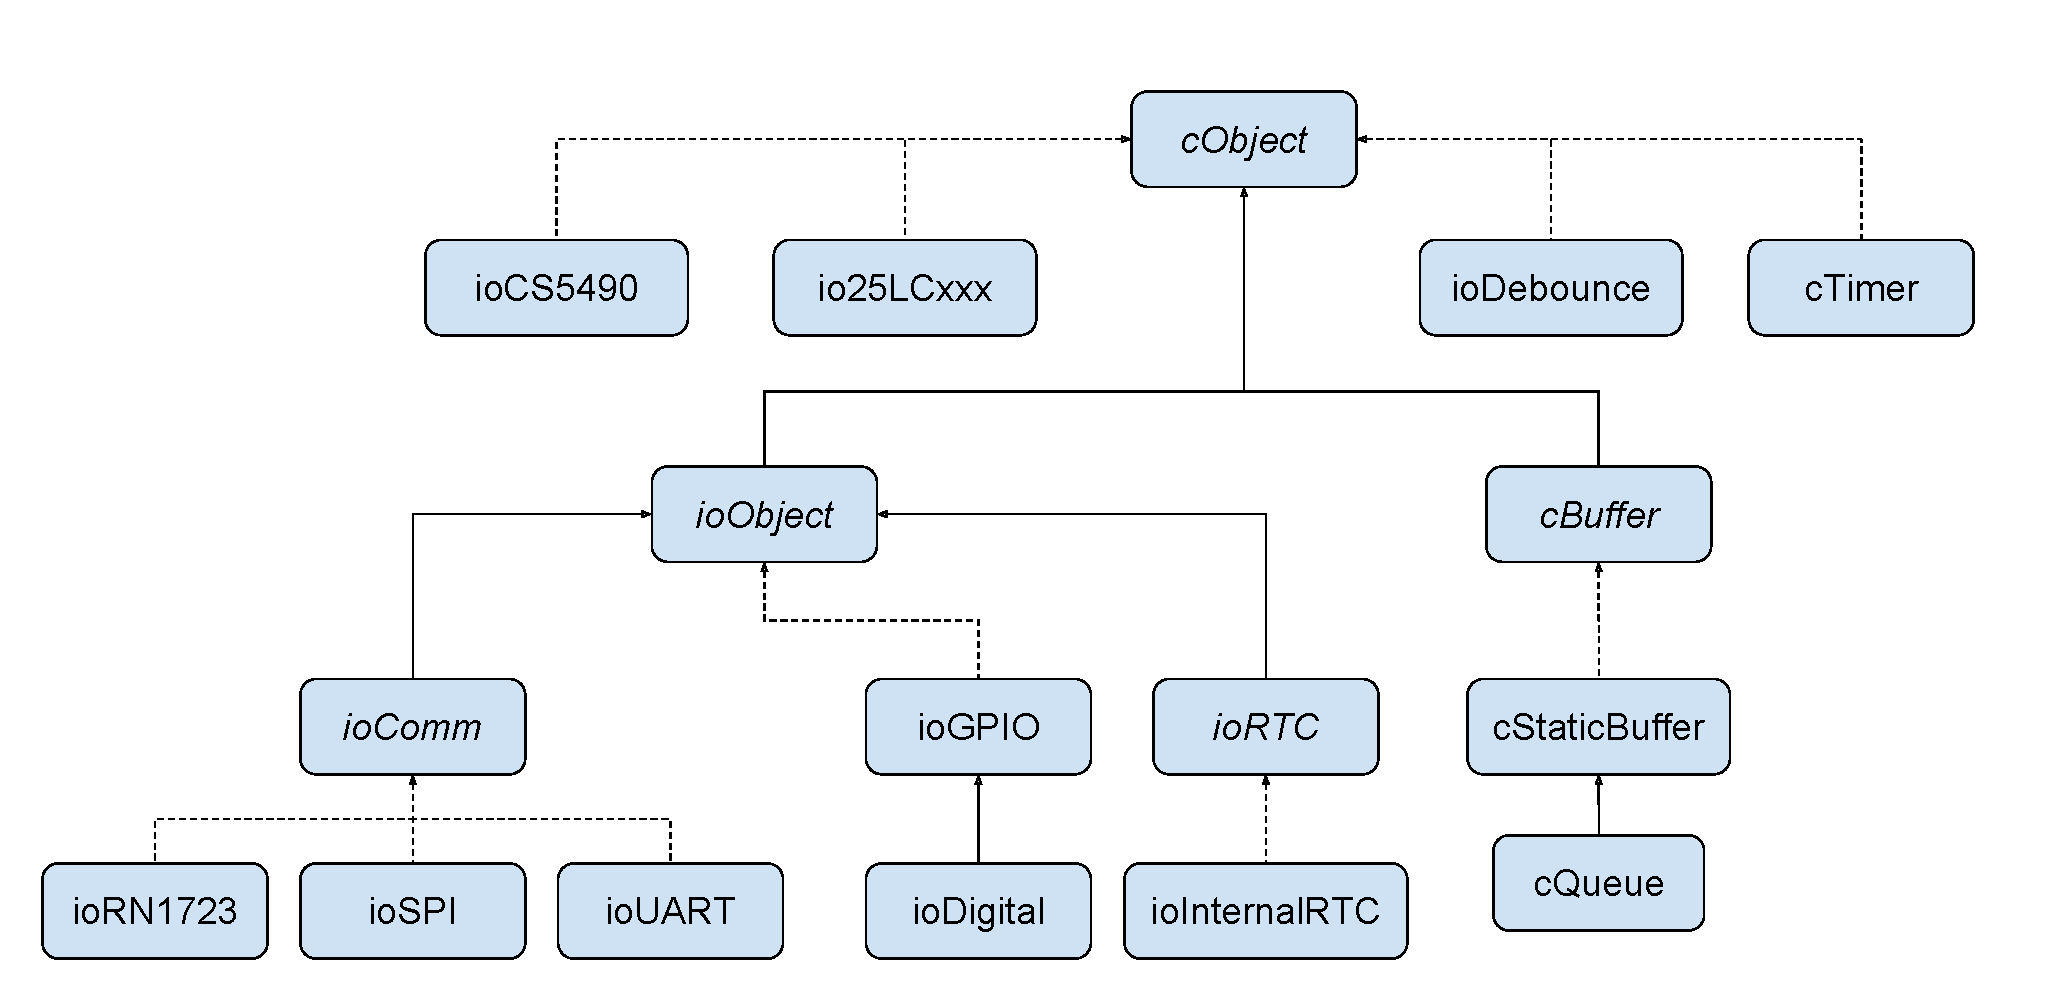
\includegraphics[width=14cm]{./Figures/3_2_3_diagrama-clases-simplificado.pdf}
	\caption{Diagrama de clases de los controladores desarrollados para el firmware.}
	\label{fig:firmware_diagrama_clases}
\end{figure}

La idea general detrás de esta forma para programar módulos de firmware se puede ver en la Figura \ref{fig:firmware_diagrama_interfaces}. Todas las clases implementadas en este trabajo parten de la interfaz \textit{cObject}. Se la llama interfaz y no clase, ya que su comportamiento es similar a las interfaces de Java: \textit{cObject} no implementa la lógica de sus métodos, sino que simplemente declara los prototipos de las funciones (esto se implementa mediante punteros a funciones). Las clases que implementen la interfaz \textit{cObject} deberán establecer la algoritmia para cada uno de los métodos contenidos en la interfaz \textit{cObject}.

\begin{figure}[h]
	\centering
	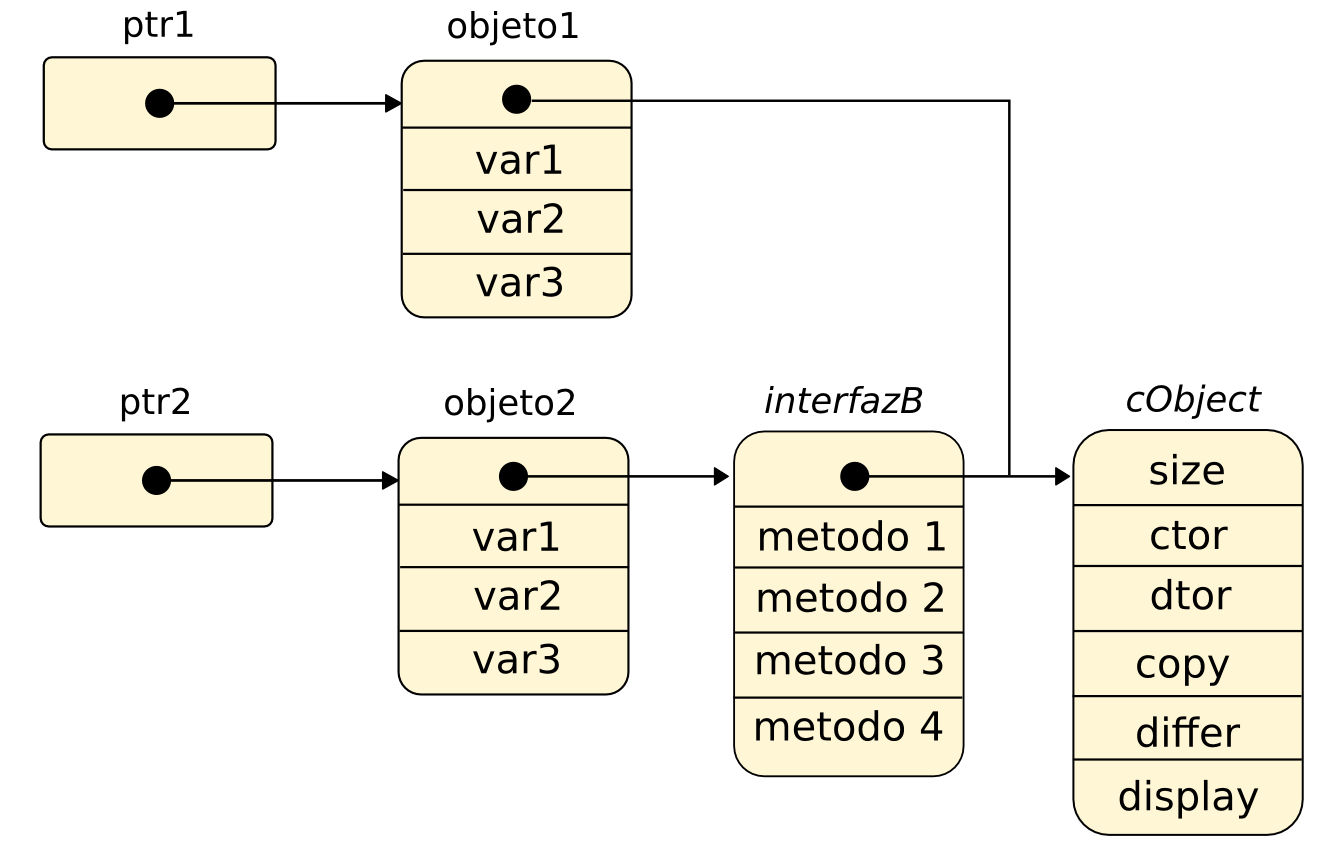
\includegraphics[width=9cm]{./Figures/3_2_3_c_orientado_objetos.png}
	\caption{Creación de interfaces y objetos en C.}
	\label{fig:firmware_diagrama_interfaces}
\end{figure}

Este comportamiento puede verse en la parte superior de la Figura \ref{fig:firmware_diagrama_interfaces}: \textit{objeto1} es una clase que implementa la  interfaz \textit{cObject}. Esta interfaz contiene los métodos básicos necesarios para cualquier otra clase: un constructor, un destructor, una función para crear una copia de un objeto, una función para determinar si dos objetos son iguales y una para mostrar el contenido del objeto de forma comprensible para un humano. Además contiene un campo \textit{size} el cual indica la cantidad de bytes que ocupa una instancia de la clase en memoria RAM.

Por lo tanto \textit{objeto1} debe implementar la lógica de todos los métodos incluidos en \textit{cObject}. Además de implementar la algoritmia, \textit{objeto1} puede contener variables que van a ser propias de cada instancia. En la Figura \ref{fig:firmware_diagrama_interfaces}, estas variables son var1, var2 y var3. Por otro lado, \textit{objeto1} puede declarar funciones que solamente puedan ser utilizadas sobre instancias de la clase \textit{objeto1}.

Finalmente \textit{ptr1} es un puntero a la instancia de \textit{objeto1}. El tipo de variable de \textit{ptr1} es \textit{void*}, es decir que la implementación de la clase queda totalmente encapsulada, ya que la aplicación que instancie a \textit{objeto1} no conocerá su estructura interna.

Con esta metodología también es posible implementar la herencia tanto de interfaces como de clases. En la parte inferior de la Figura \ref{fig:firmware_diagrama_interfaces} puede verse un ejemplo de herencia de interfaces. En este caso, la \textit{interfazB} hereda a la interfaz \textit{cObject}, agregando 3 métodos a los ya definidos por \textit{cObject}. Por lo tanto, la clase que implementa la \textit{interfazB} debe implementar todos los métodos, tanto los definidos por \textit{cObject} como los de \textit{interfazB}. En el ejemplo, esta clase es \textit{objeto2}, la cual además define 3 variables. Nuevamente \textit{ptr2} es un puntero a \textit{void} el cual apunta al área de memoria donde fue creada la instancia de \textit{objeto2}.

Como puede suponerse esta metodología de trabajo requiere además implementar alguna forma de asignación dinámica de memoria. Para este trabajo se decidió implementar un pool de memoria, el cual contiene una sencilla lógica que permite asignar, liberar y unir segmentos continuos (para reducir la fragmentación) del pool de memoria. 

Esta librería es una modificación de la descripta en \citep{an_microchip_malloc}, en la que delante de cada segmento de memoria se coloca un encabezado de dos bytes que indica si está asignado el bloque de memoria o no y la longitud del bloque. El código fuente de la librería de asignación de memoria puede encontrarse dentro de la carpeta \textit{memAlloc} en \citep{repo_firmware}.

Se debe aclarar que esta forma de trabajo no contradice la naturaleza estática del RTOS FreeOSEK. Como condición en la implementación del firmware se estableció que la creación y destrucción de los objetos únicamente se pudiera hacer en el comienzo de la aplicación. De esta forma, cuando el RTOS se encuentra funcionando no se producen más asignaciones dinámicas de memoria y el sistema se comporta como si fuera estático.

En cuanto a las clases desarrolladas se puede mencionar lo siguiente:

\begin{itemize}
\item \textit{ioObject} es una interfaz que hereda a \textit{cObject} y agrega los métodos básicos necesarios para cualquier periférico de entrada/salida: inicialización, habilitación/deshabilitación y escritura/lectura.

\item \textit{ioGPIO} es una clase que implementa a la interfaz \textit{ioObject} y que sirve como base para las clases que describen tipos más específicos de GPIOs, como por ejemplo pines digitales a través de la clase \textit{ioDigital}.

\item \textit{ioDigital} es una clase que herada a \textit{ioGPIO} e implementa la lógica para manejar los GPIO del microcontrolador LPC176x como pines digitales, tanto entradas como salidas.

\item \textit{ioRTC} es una interfaz que hereda a \textit{ioObject} y los métodos básicos necesarios para manejar relojes de tiempo real, tanto internos al microcontrolador, como externos: reset del reloj, lectura y escritura de la hora y fecha.

\item \textit{ioInternalRTC} es una clase que implementa la interfaz \textit{ioRTC} y permite configurar y consultar el RTC interno del microcontrolador LPC176x.

\item \textit{ioComm} es una interfaz que hereda a \textit{ioObject} y agrega los métodos básicos para las clases que modelen periféricos de comunicación: lectura y escritura de cadenas de bytes, determinación de espacio disponible en buffers, habilitación/deshabilitación/consulta de interrupciones.

\item \textit{ioUART} es una clase que implementa la interfaz \textit{ioComm} y que permite manejar las UARTs del microcontrolador LPC176x y las interrupciones relacionadas con estos periféricos. Además agrega el manejo de buffers de recepción y transmisión. La comunicación se puede implementar tanto de forma bloqueante como mediante interrupciones.

\item \textit{ioSPI} es una clase que implementa la interfaz \textit{ioComm} y que permite manejar los SPI del microcontrolador LPC176x. La comunicación es siempre bloqueante.

\item \textit{ioRN1723} es una clase que implementa la interfaz \textit{ioComm} y que permite manejar el módulo WiFi RN1723. Implementa la lógica para poder configurar el módulo, iniciar el modo WPS y AP y manejar las conexiones TCP. Esta clase requiere de otras clases para poder funcionar: \textit{ioUART} para implementar la comunicación con el módulo, \textit{ioDigital} para manejar los pines de reset y GPIO del módulo, \textit{cQueue} para implementar los buffers de recepción y transmisión, \textit{cTimer} para determinar eventos de timeout del módulo y de las conexiones TCP.

\item \textit{cBuffer} es una interfaz que herada a \textit{cObject} y agrega los métodos necesarios para las clases que modelen contenedores de datos: agregado y borrado de elementos, consulta de elementos, consulta de espacio libre, limpieza del contenedor, etc.

\item \textit{cStaticBuffer} es una clase que implementa la interfaz \textit{cBuffer} y que sirve como base para todas las clases que implementen contenedores de tamaño fijo.

\item \textit{cQueue} es una clase que hereda a \textit{cStaticBuffer} e implementa la lógica de una cola, es decir un contenedor de tipo FIFO (First In First Out, primero entra primero sale). Puede contener objetos de cualquier cantidad de bytes pero deben ser todos del mismo tipo.

\item \textit{ioCS5490} es una clase que implementa la interfaz \textit{cObject} que permite manejar el front-end analógico CS5490. Implementa la lógica para poder leer/escribir registros y contiene las variables necesarias para obtener las mediciones eléctricas. Esta clase depende de otras para poder funcionar: \textit{ioUART} para implementar la comunicación con el módulo y \textit{ioDigital} para los pines de reset y de pulsos de energía consumida.

\item \textit{io25LCxxx} es una clase que implementa la interfaz \textit{cObject} que permite manejar memorias EEPROM de la línea 25LC fabricadas por Microchip. Una instancia de esta clase puede ser configurada para escribir/leer/borrar datos de memorias de distintas capacidades, desde 32kbit  hasta 1Mbit. Esta clase depende de \textit{ioSPI} para implementar la comunicación con la memoria externa.

\item \textit{ioDebounce} es una clase que implementa la interfaz \textit{cObject} y permite ejecutar la lógica de un anti-rebote sobre una instancia de la clase \textit{ioDigital}.

\item \textit{ioTimer} es una clase que implementa la interfaz \textit{cObject} y permite implementar timers sencillos y detectar cuando vencen mediante polling. La base de tiempo debe ser establecida por el usuario de la clase \textit{ioTimer}.

\end{itemize}

El código fuente de todas las interfaces y clases puede encontrarse en la carpeta \textit{cObject} en \citep{repo_firmware}. Dentro de esta carpeta también puede encontrarse un diagrama de clases completo (\textit{class\_diag\_cObject.dia}) con los métodos y variables que define cada clase e interfaz.


\subsection{Protocolo de comunicación}
\label{subsection:protocolo}

Para poder intercambiar comandos y respuestas entre la aplicación móvil y los Smart Plugs fue necesario implementar un protocolo de comunicación. Este protocolo está por encima de TCP, el cual se usa para establecer la conexión y proveer la de retransmisiones y corrección de errores. La trama del protocolo desarrollado puede verse en la Figura \ref{fig:formato_trama}. 

\begin{figure}[h]
	\centering
	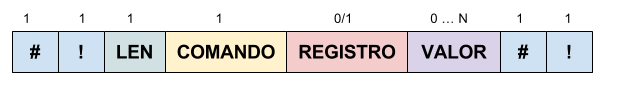
\includegraphics[width=13cm]{./Figures/3_2_4_formato_trama.png}
	\caption{Formato de la trama del protocolo desarrollado para comunicar la aplicación móvil con los Smart Plugs.}
	\label{fig:formato_trama}
\end{figure}

Cada trama va a comenzar y a terminar con los caracteres \textit{\#!}, lo cual facilita la recepción. Además están los siguientes campos:

\begin{itemize}
\item LEN: indica la cantidad de bytes de la trama desde el campo COMANDO hasta los caracteres \textit{\#!} finales incluidos.
\item COMANDO: es un byte que indica el código del comando que se está enviando. En la Tabla \ref{tab:comandos_trama} pueden verse todos los posibles valores para este campo.
\item REGISTRO: indica el registro que se quiere leer, escribir o reiniciar. Es un campo opcional, de acuerdo al comando. En la Tabla \ref{tab:registros_trama} puede verse un resumen de los registros disponibles.
\item VALOR: indica el valor que se leyó o se quiere escribir en un registro. Este campo va a variar de acuerdo al registro manipulado. En algunos registros, el campo valor será los 4 bytes de un float, en otros registros será los bytes de una cadena de caracteres, etc. Es responsabilidad del receptor interpretar los bytes de este campo de acuerdo al registro.
\end{itemize}



\begin{table}[h]
	\centering
	\caption[Comandos disponibles en el protocolo]{Comandos disponibles en el protocolo.}
	\begin{tabular}{c c p{6cm}}    
		\toprule
		\textbf{Comando} 	 & \textbf{Descipción}  & \textbf{Notas} \\
		\midrule
		0x01  & GET(registro)  				& Pide el valor de un registro \\		
		0x02  & SET(registro, valor)  		& Escribe el valor de un registro \\
		0x10  & NODE\_ON()  					& Enciende la carga manejada por el Smart Plug \\
		0x11  & NODE\_OFF()  				& Apaga la carga manejada por el Smart Plug \\
		0x20  & RESET(registro)  			& Reinicia el valor del registro \\
		0x30  & RESP\_GET(registro, valor)  	& Informa el valor del registro pedido \\
		0x31  & RESP\_SET(registro, valor)  	& Confirma el valor escrito en el registro \\
		0x32  & RESP\_RESET(registro)  		& Confirma que el valor del registro fue reiniciado \\
		0x33  & RESP\_NODE\_ON()  			& Confirma que la carga fue encendida \\
		0x34  & RESP\_NODE\_OFF()  			& Confirma que la carga fue apagada \\
		\bottomrule
		\hline
	\end{tabular}
	\label{tab:comandos_trama}
\end{table}

\begin{table}[h]
	\centering
	\caption[Resumen de los registros disponibles en el protocolo]{Resumen de los registros disponibles en el protocolo.}
	\begin{tabular}{c p{5cm} p{6cm}}    
		\toprule
		\textbf{Comando} 	 & \textbf{Descripción}  & \textbf{Notas} \\
		\midrule
		0x01 a 0x08  	& Registros de mediciones eléctricas  	& Incluye: tensión eficaz, corriente eficaz, factor de potencia, frecuencia, potencia activa, energía total consumida, etc. \\		
		0x10  			& DEVICE\_ID  							& Nombre del dispositivo. Es el nombre que identifica al Smart Plug en la aplicación móvil. \\
		0x15  			& LOAD\_STATE  							& Indica si la carga está encendida o apagada. \\
		0x20 a 022F  	& Registros de programación horaria  	& Es un conjunto de registros que contiene la hora de encendido y la de apagado de la carga para cada día de la semana. \\
		0x30  			& PER\_HOUR\_ENERGY  						& Contiene las 24 mediciones de energía consumida por hora de una determinada fecha. \\
		0x31  			& PER\_HOUR\_ACTIVE\_POWER  				& Contiene las 24 mediciones de potencia activa promedio por hora de una determinada fecha. \\
		\bottomrule
		\hline
	\end{tabular}
	\label{tab:registros_trama}
\end{table}

Una característica a destacar es que este protocolo es de lazo cerrado. Para cualquier comando hay una respuesta que indica que ese comando fue recibido por el Smart Plug. Esta característica es usada por la aplicación móvil, en la cual cuando el usuario cambia un valor de configuración del Smart Plug, el cambio no se muestra en la pantalla de la aplicación hasta haber recibido la respuesta del comando enviado. De esta forma se asegura que el comando se haya recibido.

La forma en que se implementó el protocolo permite en un futuro agregar nuevos comandos y registros. Solamente será necesario agregar estos nuevos campos en el firmware del Smart Plug y en la aplicación móvil.


\subsection{Uso de los comandos}

A continuación se muestran los distintos escenarios que se pueden dar utilizando el protocolo desarrollado.

En el caso de leer un registro se tiene la secuencia mostrada en la Figura \ref{fig:comunicacion_get}. En este ejemplo, se quiere obtener el valor (campo COMANDO = 0x01 - GET) del registro de la potencia activa (campo REGISTRO = 0x05). Cuando la tarea taskWiFi en el Smart Plug recibe esta petición le pide el valor actual de la potencia activa a la tarea taskMeter y devuelve el valor con el comando 0x30 (RESP\_GET).

\begin{figure}[h]
	\centering
	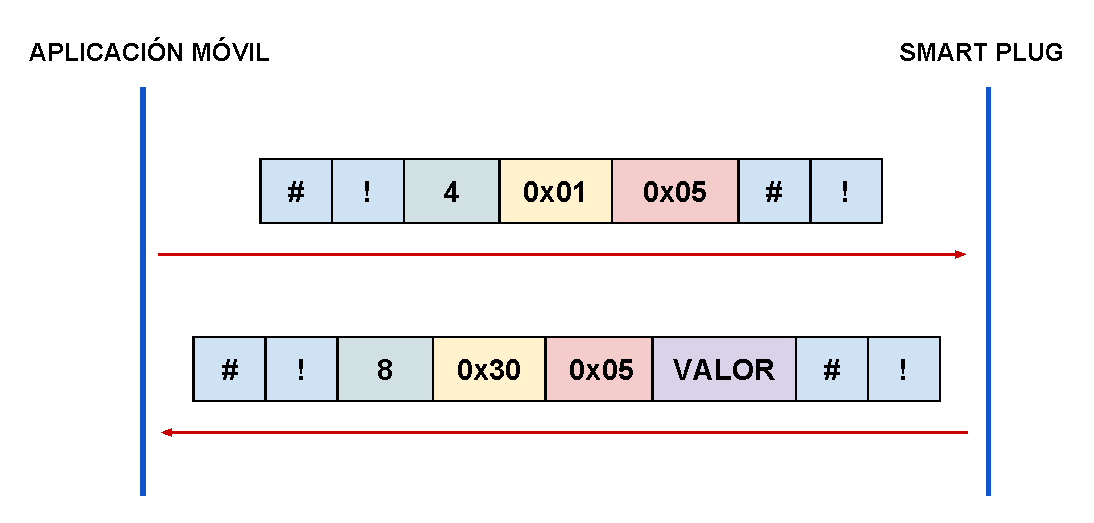
\includegraphics[width=14cm]{./Figures/3_2_5_comunicacion_GET.pdf}
	\caption{Diagrama de comunicación del comando \textit{GET}.}
	\label{fig:comunicacion_get}
\end{figure}

Como se mencionó anteriormente, el campo valor se debe interpretar de distinta forma de acuerdo al registro que se quiera leer. En el caso del registro ACTIVE\_POWER (0x05) el campo valor va a contener los 4 bytes del float de la potencia activa ordenados en formato \textit{Big Endian}.

Cuando se quiere escribir un registro en el Smart Plug, se debe enviar un comando SET y el nuevo valor del registro. En la Figura \ref{fig:comunicacion_set} puede verse la secuencia. En este ejemplo, la aplicación móvil quiere cambiar el registro de la hora de encendido de la carga para los días lunes (REGISTRO = 0x20), con la hora 12:10. 

\begin{figure}[h]
	\centering
	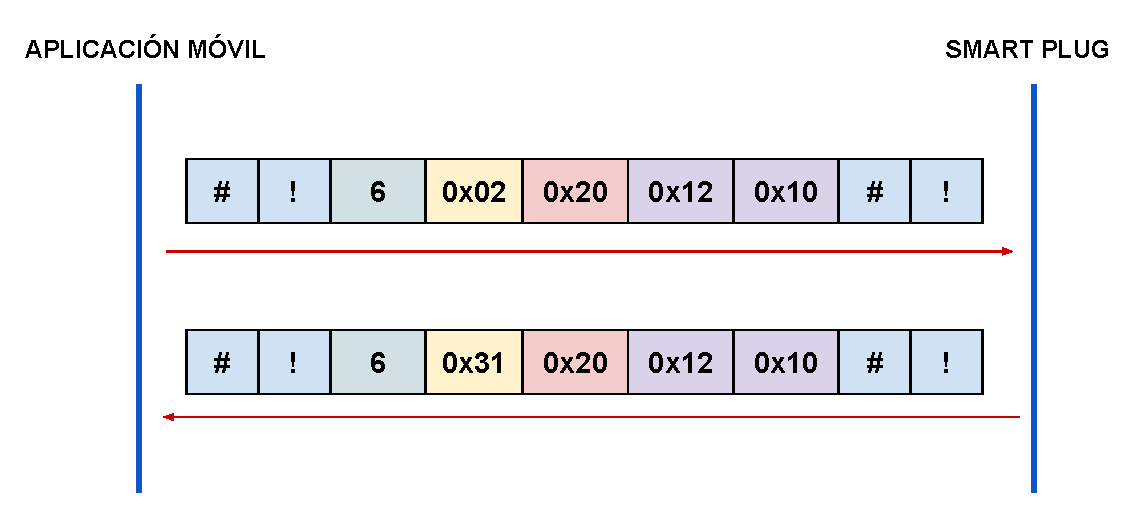
\includegraphics[width=14cm]{./Figures/3_2_5_comunicacion_SET.pdf}
	\caption{Diagrama de comunicación del comando \textit{SET}.}
	\label{fig:comunicacion_set}
\end{figure}

Cuando taskWiFi recibe este comando, escribe el nuevo valor para el registro en la EEPROM, genera la trama de respuesta con el comando RESP\_SET (0x31) y devuelve el valor que fue cargado en el registro. El hecho de devolver el mismo valor que recibió ayuda a la aplicación móvil a actualizar los datos en sus registros internos.

En este caso se puede ver que el campo valor se debe interpretar como dos bytes, en el cual el primero indica la hora y el segundo los minutos del encendido de la carga.

Además de escribir un valor determinado en un registro, el protocolo permite indicar que se debe reiniciar el valor de un registro. Para lograr esto se debe utilizar el comando RESET (0x20) y el registro que se quiere reiniciar. En el ejemplo de la Figura \ref{fig:comunicacion_reset} se puede ver cómo se quiere reiniciar el nombre del dispositivo (campo REGISTRO = 0x10).

\begin{figure}[h]
	\centering
	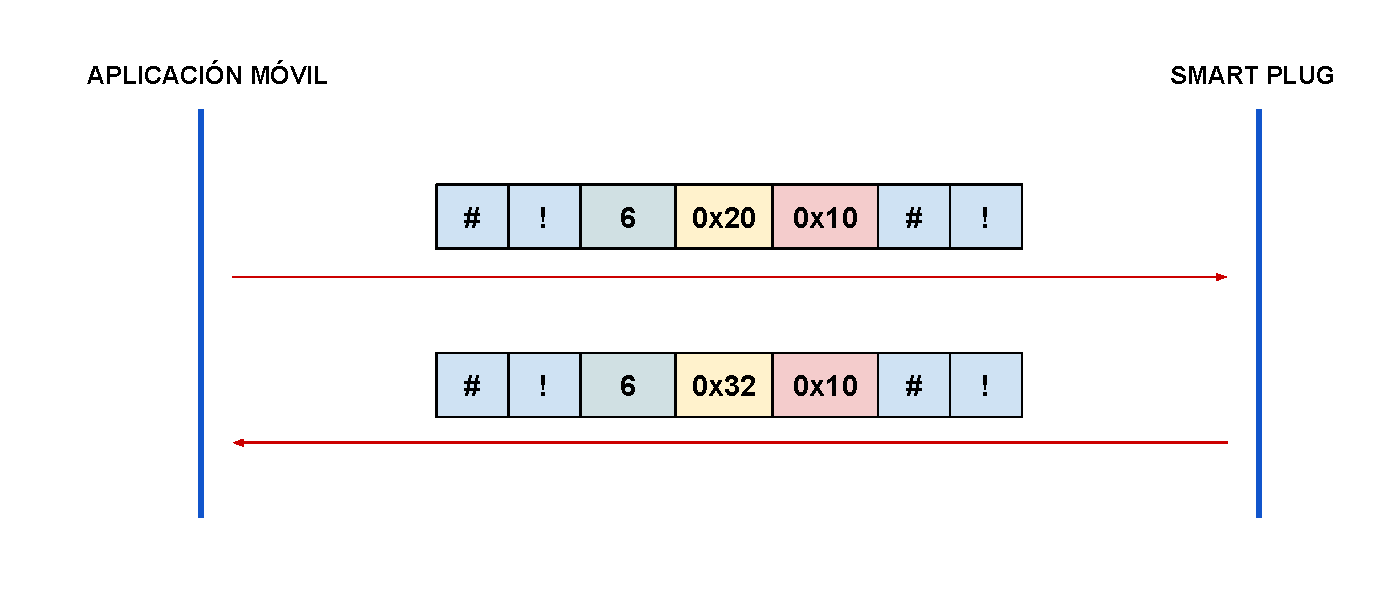
\includegraphics[width=14cm]{./Figures/3_2_5_comunicacion_RESET.pdf}
	\caption{Diagrama de comunicación del comando \textit{RESET}.}
	\label{fig:comunicacion_reset}
\end{figure}

Cuando la tarea taskWiFi recibe este comando escribe el valor de fábrica asociado al registro en la EEPROM. Por ejemplo, para el caso del nombre de dispositivo, el valor de fábrica es \textit{Smart Plug}. Sin embargo, cada registro tiene un valor de fábrica distinto. Una vez reiniciado el registro, el Smart Plug genera una trama de respuesta con el comando RESP\_RESET (0x32) acompañado del registro modificado.

Finalmente existen dos comandos dedicados al control de la carga conectada al Smart Plug. Estos son NODE\_ON (0x10) y NODE\_OFF (0x11). Mediante estos comandos, se le indica al Smart Pug que encienda o apague la carga. En la Figura \ref{fig:comunicacion_node} puede verse la secuencia cuando se envían estos comandos.

\begin{figure}[h]
	\centering
	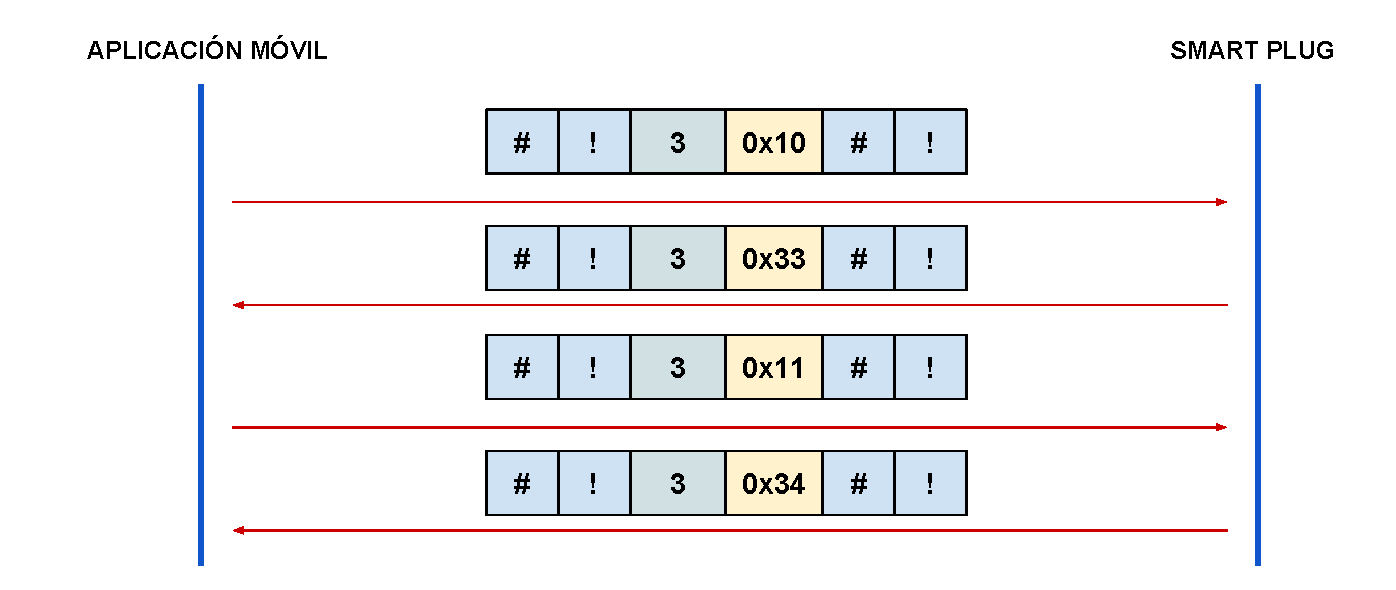
\includegraphics[width=14cm]{./Figures/3_2_5_comunicacion_NODE.pdf}
	\caption{Diagrama de comunicación de los comandos \textit{NODE ON} y \textit{NODE OFF}.}
	\label{fig:comunicacion_node}
\end{figure}

La tarea taskWiFi al recibir estos comandos genera un evento y la tarea taskSmartPlug enciende o apaga la carga a partir del evento recibido. Hecho esto, se devuelve una trama con el comando RESP\_NODE\_ON (0x33) o RESP\_NODE\_OFF (0x34) para que la aplicación móvil tenga la confirmación de que la carga fue conmutada.


\section{Aplicación Android}
\label{section:app}

\subsection{Maqueta de la aplicación}
\label{subsec:app_wireframe}

Antes de comenzar con el diseño de la lógica de la aplicación, fue necesario determinar la forma en la que se iban a presentar los datos al usuario. Para esto se recurrió al uso de una maqueta, en la cual se muestran las pantallas de las que estará compuesta la aplicación y la interacción que hay entre ellas. Cada una de las pantallas presenta el aspecto que realmente debe tener en la aplicación pero no describe la forma en que se debe implementar la lógica.

En la Figura \ref{fig:app_wireframe} puede verse la maqueta completa de la aplicación. La líneas rojas muestran la interacción entre las pantallas y las violetas son comentarios que clarifican el funcionamiento de la pantalla.

\begin{figure}[!h]
	\centering
	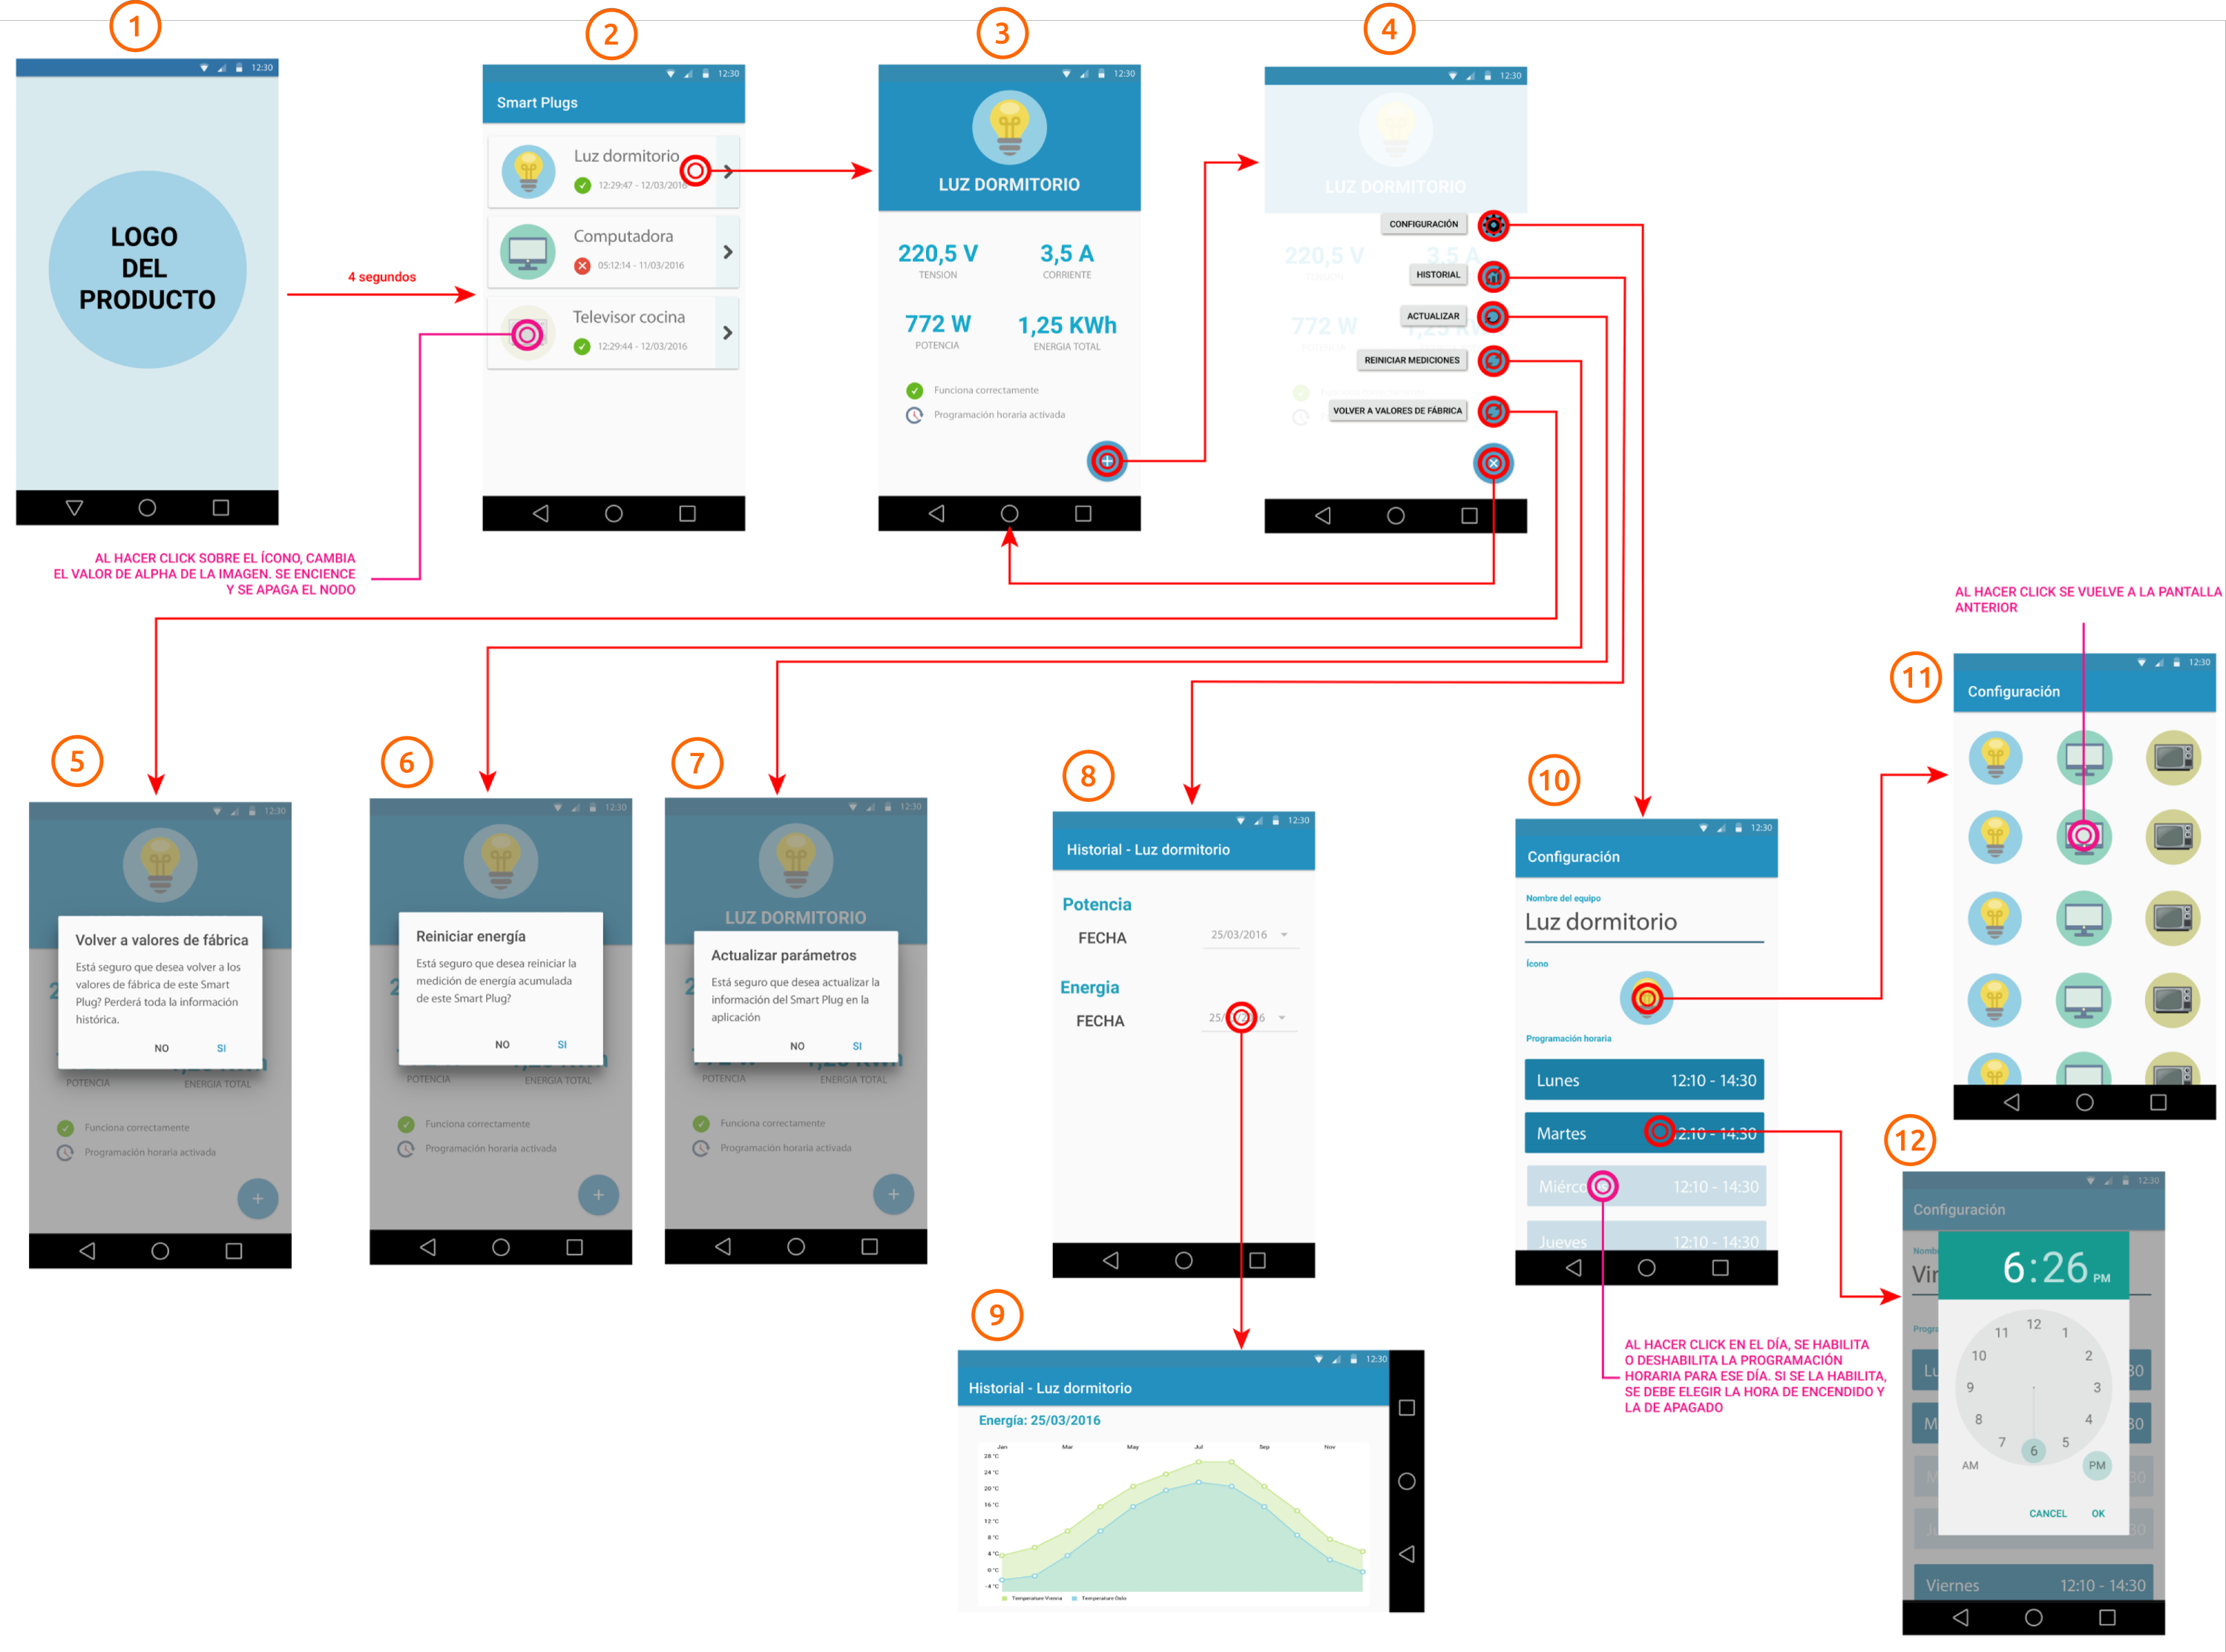
\includegraphics[width=18cm, angle=90]{./Figures/3_3_1_app_wireframe.png}
	\caption{Maqueta de la aplicación móvil.}
	\label{fig:app_wireframe}
\end{figure}

A continuación se describe brevemente el funcionamiento de la aplicación desde el punto de vista del usuario:

\begin{itemize}
\item  Pantalla 1 (parte izquierda de la Figura \ref{fig:app_wireframe_1}): la aplicación comienza con un \textit{splash screen}, es decir, una pantalla que muestra el logo y el nombre de la aplicación durante unos segundos y luego da paso a la siguiente pantalla.

\item Pantalla 2 (parte central de la Figura \ref{fig:app_wireframe_1}): luego del \textit{splash screen} se muestra una lista con todos los Smart Plugs que se encontraron en la red WiFi. Como se explicará en la Subsección \ref{subsec:arquitectura_app}, cada Smart Plug se identifica periódicamente dentro de la red WiFi. Estos mensajes periódicos son capturados por la aplicación y en el caso de detectar un Smart Plug que no conocía, lo agregará en la lista. La forma de identificar unívocamente a cada Smart Plug es mediante un número único que se graba en la EEPROM del equipo durante el proceso de fabricación. Este es un número de seis dígitos que es informado en los mensajes UDP periódicos.

Cada uno de los elementos de la lista representa a un Smart Plug. Se va a mostrar el nombre del dispositivo, el estado de la comunicación mediante un tilde verde o una cruz roja y la fecha y hora de la última comunicación exitosa que hubo con ese Smart Plug. Además se muestra un ícono que permite identificar de forma sencilla el dispositivo que realmente está controlando el Smart Plug. 

Sin embargo, el ícono no cumple únicamente una función pictórica: si se lo presiona se puede conmutar el estado de la carga. Más aún, la opacidad del ícono indica el estado actual de la misma: cuando se lo muestra semi-transparente la carga está apagada y cuando se lo muestra sin transparencia, está encendida.

\item Pantalla 3 (parte derecha de la Figura \ref{fig:app_wireframe_1}): cuando en la pantalla 2 se presiona alguno de los Smart Plugs de la lista, la aplicación muestra una vista de detalle del mismo. En esta se volverá a mostrar el ícono asociado al Smart Plug, su nombre, el estado de la comunicación y la fecha y hora de la última comunicación exitosa. Pero además de estos datos se indicarán las últimas mediciones recibidas desde el equipo. Estas mediciones incluyen: tensión eficaz, corriente eficaz, potencia activa y energía total consumida. Estos datos son actualizados periódicamente, aún cuando la aplicación se encuentre cerrada.

Por otro lado, en esta vista de detalle se encuentra presente, en la esquina inferior derecha de la pantalla, un botón de acción flotante (floating action button) el cual permite acceder a más opciones para gestionar el Smart Plug seleccionado.


\begin{figure}[!h]
	\centering
	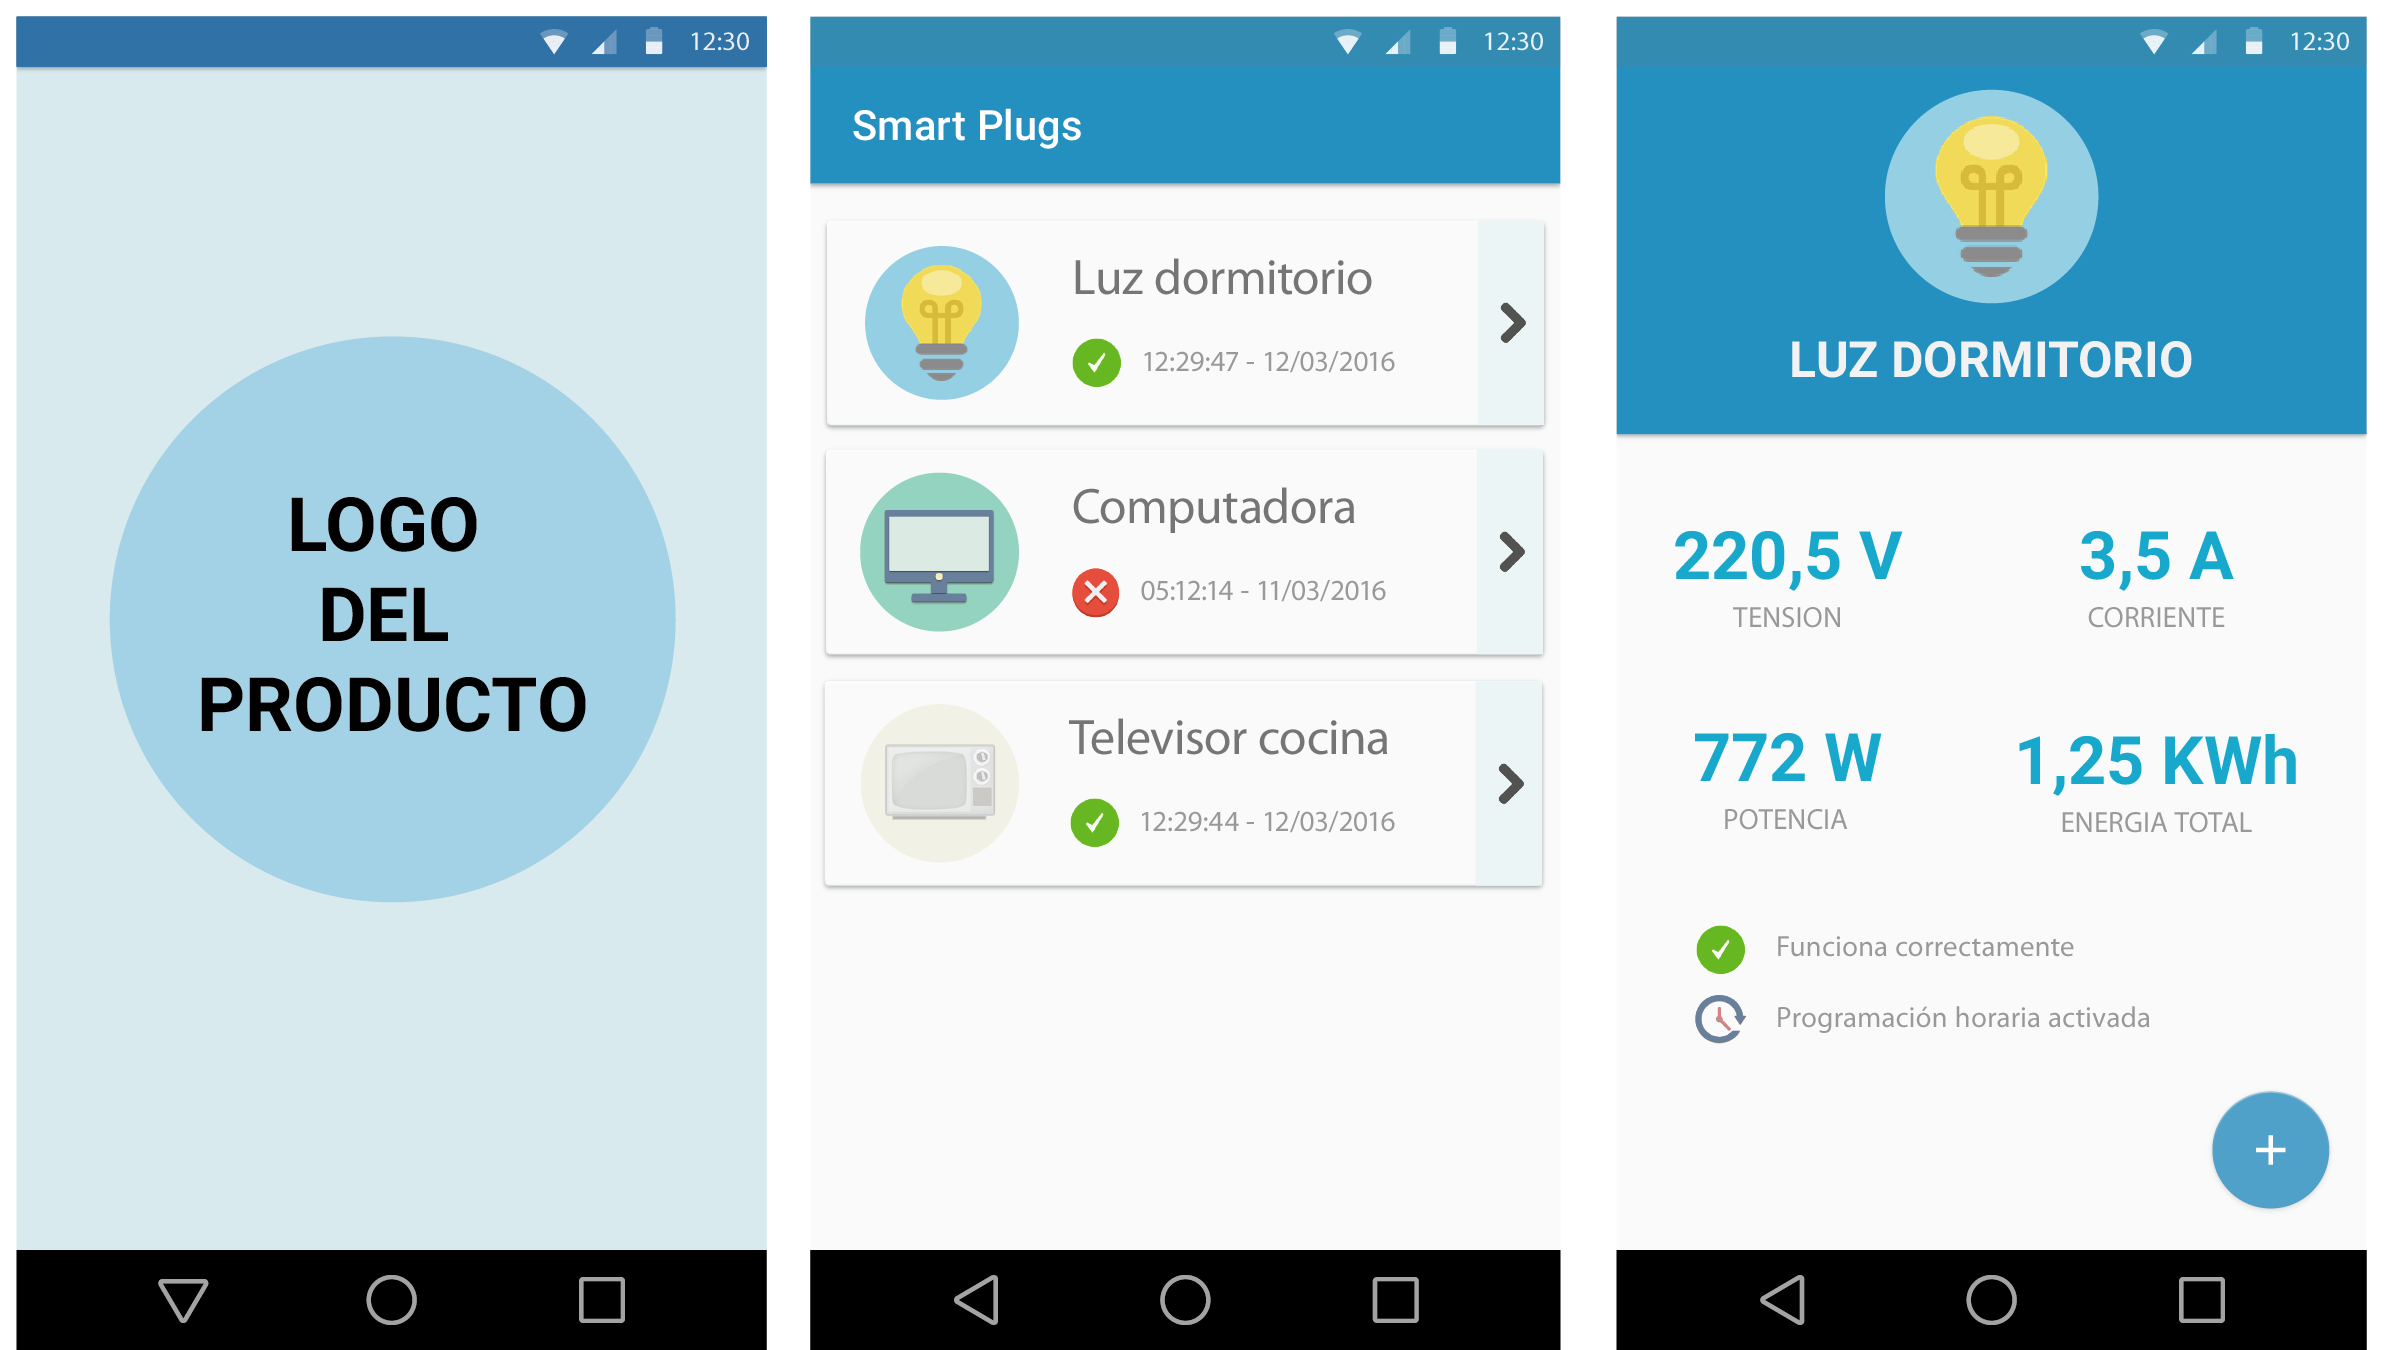
\includegraphics[width=14cm]{./Figures/3_3_1_app_wireframe_1.png}
	\caption{Detalle de la maqueta, pantallas 1, 2 y 3.}
	\label{fig:app_wireframe_1}
\end{figure}


\item Pantalla 4: cuando se presiona el botón de acción flotante se despliega un menú el cual incluye la siguiente opciones: Configuración, Historial, Actualizar, Reiniciar mediciones y Volver a valores de fábrica.

\item Pantalla 5 (parte izquierda de la Figura \ref{fig:app_wireframe_2}): si se presiona la opción de Volver a valores de fábrica, se le preguntará al usuario si confirma que quiere realizar esta acción. En caso afirmativo se le enviará al Smart Plug el comando correspondiente el cual volverá a sus valores de fábrica, los cuales consisten en:

\begin{itemize}
\item Nombre del dispositivo: Smart Plug.
\item Programación horaria de encendido/apagado deshabilitada.
\item Se reinicia el registro la energía consumida.
\item Se eliminan las mediciones históricas de potencia activa y energía consumida por hora, tanto en el Smart Plug como en la aplicación.
\end{itemize}

\item Pantalla 6 (parte central de la Figura \ref{fig:app_wireframe_2}): si se presiona la opción Reiniciar mediciones, se le preguntará al usuario si confirma que quiere realizar la acción. En caso afirmativo, se enviarán los comandos correspondientes al Smart Plug. Cuando se realiza esta acción se reiniciará el registro de la energía consumida y se eliminarán las mediciones históricas de potencia activa y energía consumida por hora. 

Se decidió incorporar esta opción para ayudar en los casos en los que, por ejemplo, se cambia la carga que está controlando el Smart Plug, por lo que se desea eliminar los registros de la anterior carga ya que podrían llevar a confusiones en la interpretación de los datos.

\item Pantalla 7 (parte derecha de la Figura \ref{fig:app_wireframe_2}): cuando se presiona la opción Actualizar, una caja de diálogo le preguntará al usuario si confirma la acción. En caso afirmativo, se forzará el proceso de actualización de los datos del Smart Plug, es decir, se le pedirán las últimas mediciones, sus parámetros de configuración y sus mediciones históricas para actualizar la información en la aplicación. Este comando es útil cuando se necesita conocer la información actual, por ejemplo, de una medición y no se puede esperar hasta la próxima consulta periódica que realiza la aplicación.


\begin{figure}[!h]
	\centering
	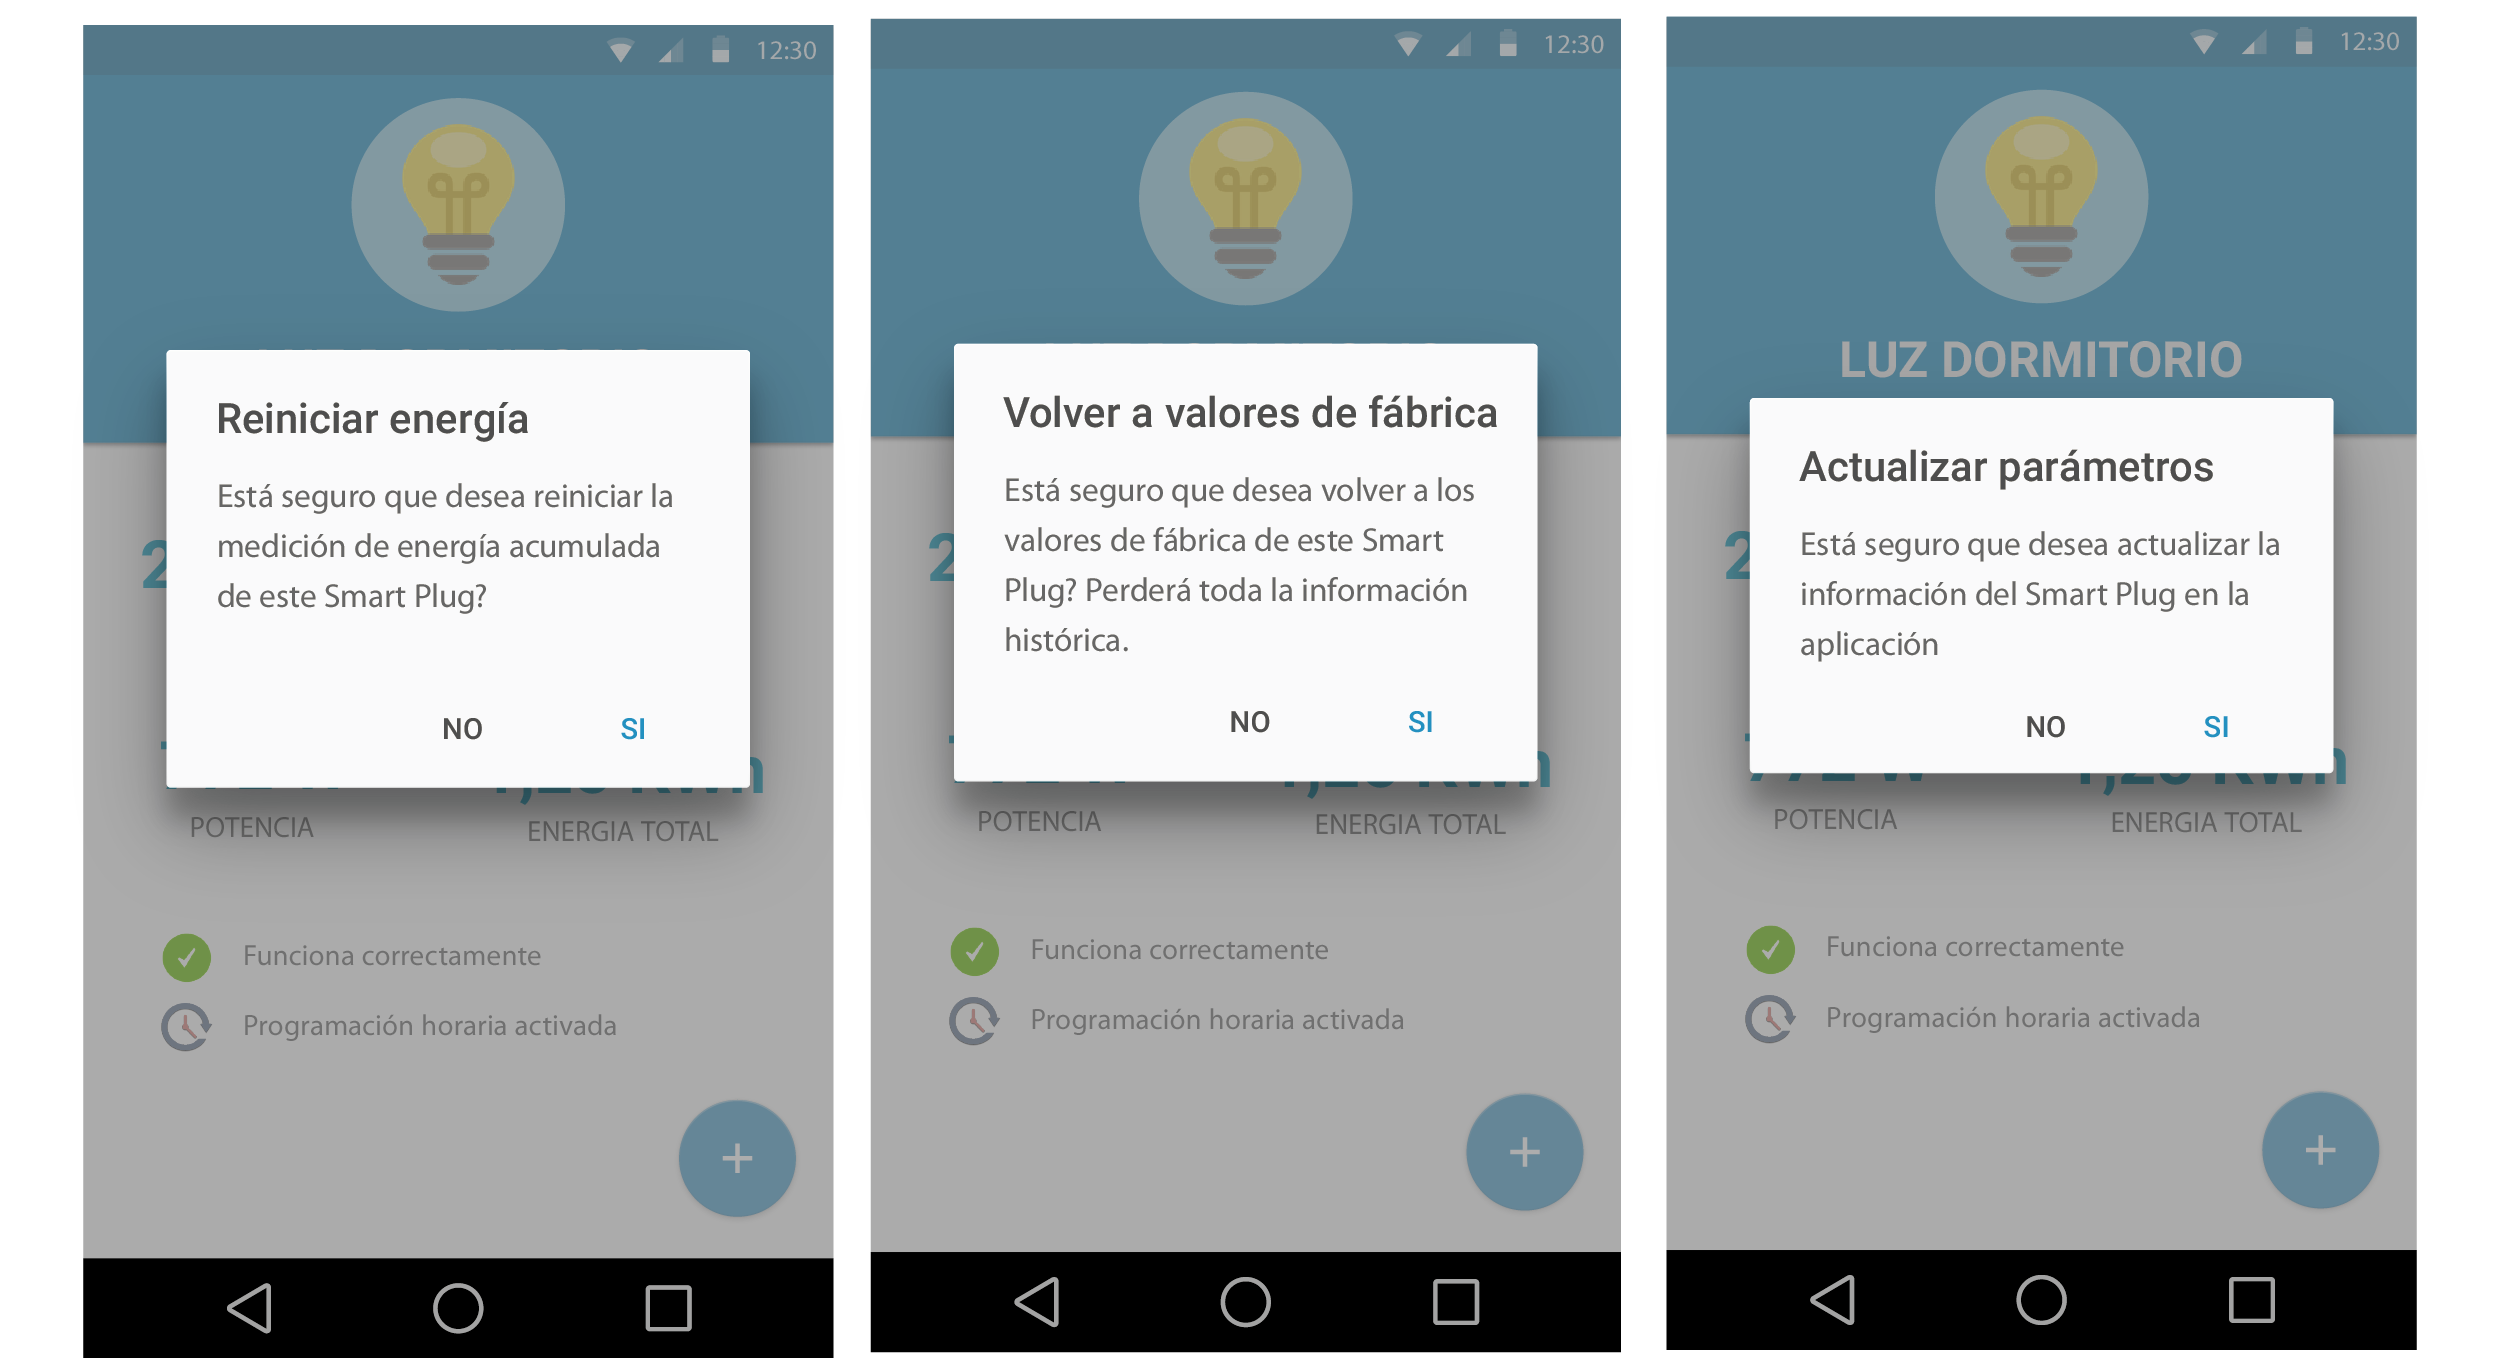
\includegraphics[width=14cm]{./Figures/3_3_1_app_wireframe_2.png}
	\caption{Detalle de la maqueta, pantallas 5, 6 y 7.}
	\label{fig:app_wireframe_2}
\end{figure}


\item Pantalla 8 (parte izquierda de la Figura \ref{fig:app_wireframe_3}): al presionar la opción Historial se accede a todas las mediciones históricas que se recibieron desde el Smart Plug. Este historial consiste en las mediciones que realizó en cada hora del día, tanto de la potencia activa promedio como de la energía consumida. En esta pantalla se podrá elegir el día que se quiere ver y el parámetro que se desea consultar mediante dos listas de fechas. Se debe aclarar que aunque el Smart Plug retenga las mediciones de los últimos 7 días, la aplicación puede retener hasta 20 días.

\item Pantalla 9 (parte derecha de la Figura \ref{fig:app_wireframe_3}): cuando se elije una fecha, la pantalla gira para mejorar la visualización de los datos en forma de gráfico. En este gráfico se va a representar la potencia activa por hora (en Watt) vs la hora del día o la energía consumida por hora (en kWh) vs la hora del día. Se puede realizar zoom y desplazarse por el gráfico arrastrando el dedo.

Estos gráficos representan una de las características distintivas de este producto, ya que permite visualizar de forma sencilla mediciones que pueden ser aprovechadas para conocer el consumo de un determinado aparato eléctrico.


\begin{figure}[!h]
	\centering
	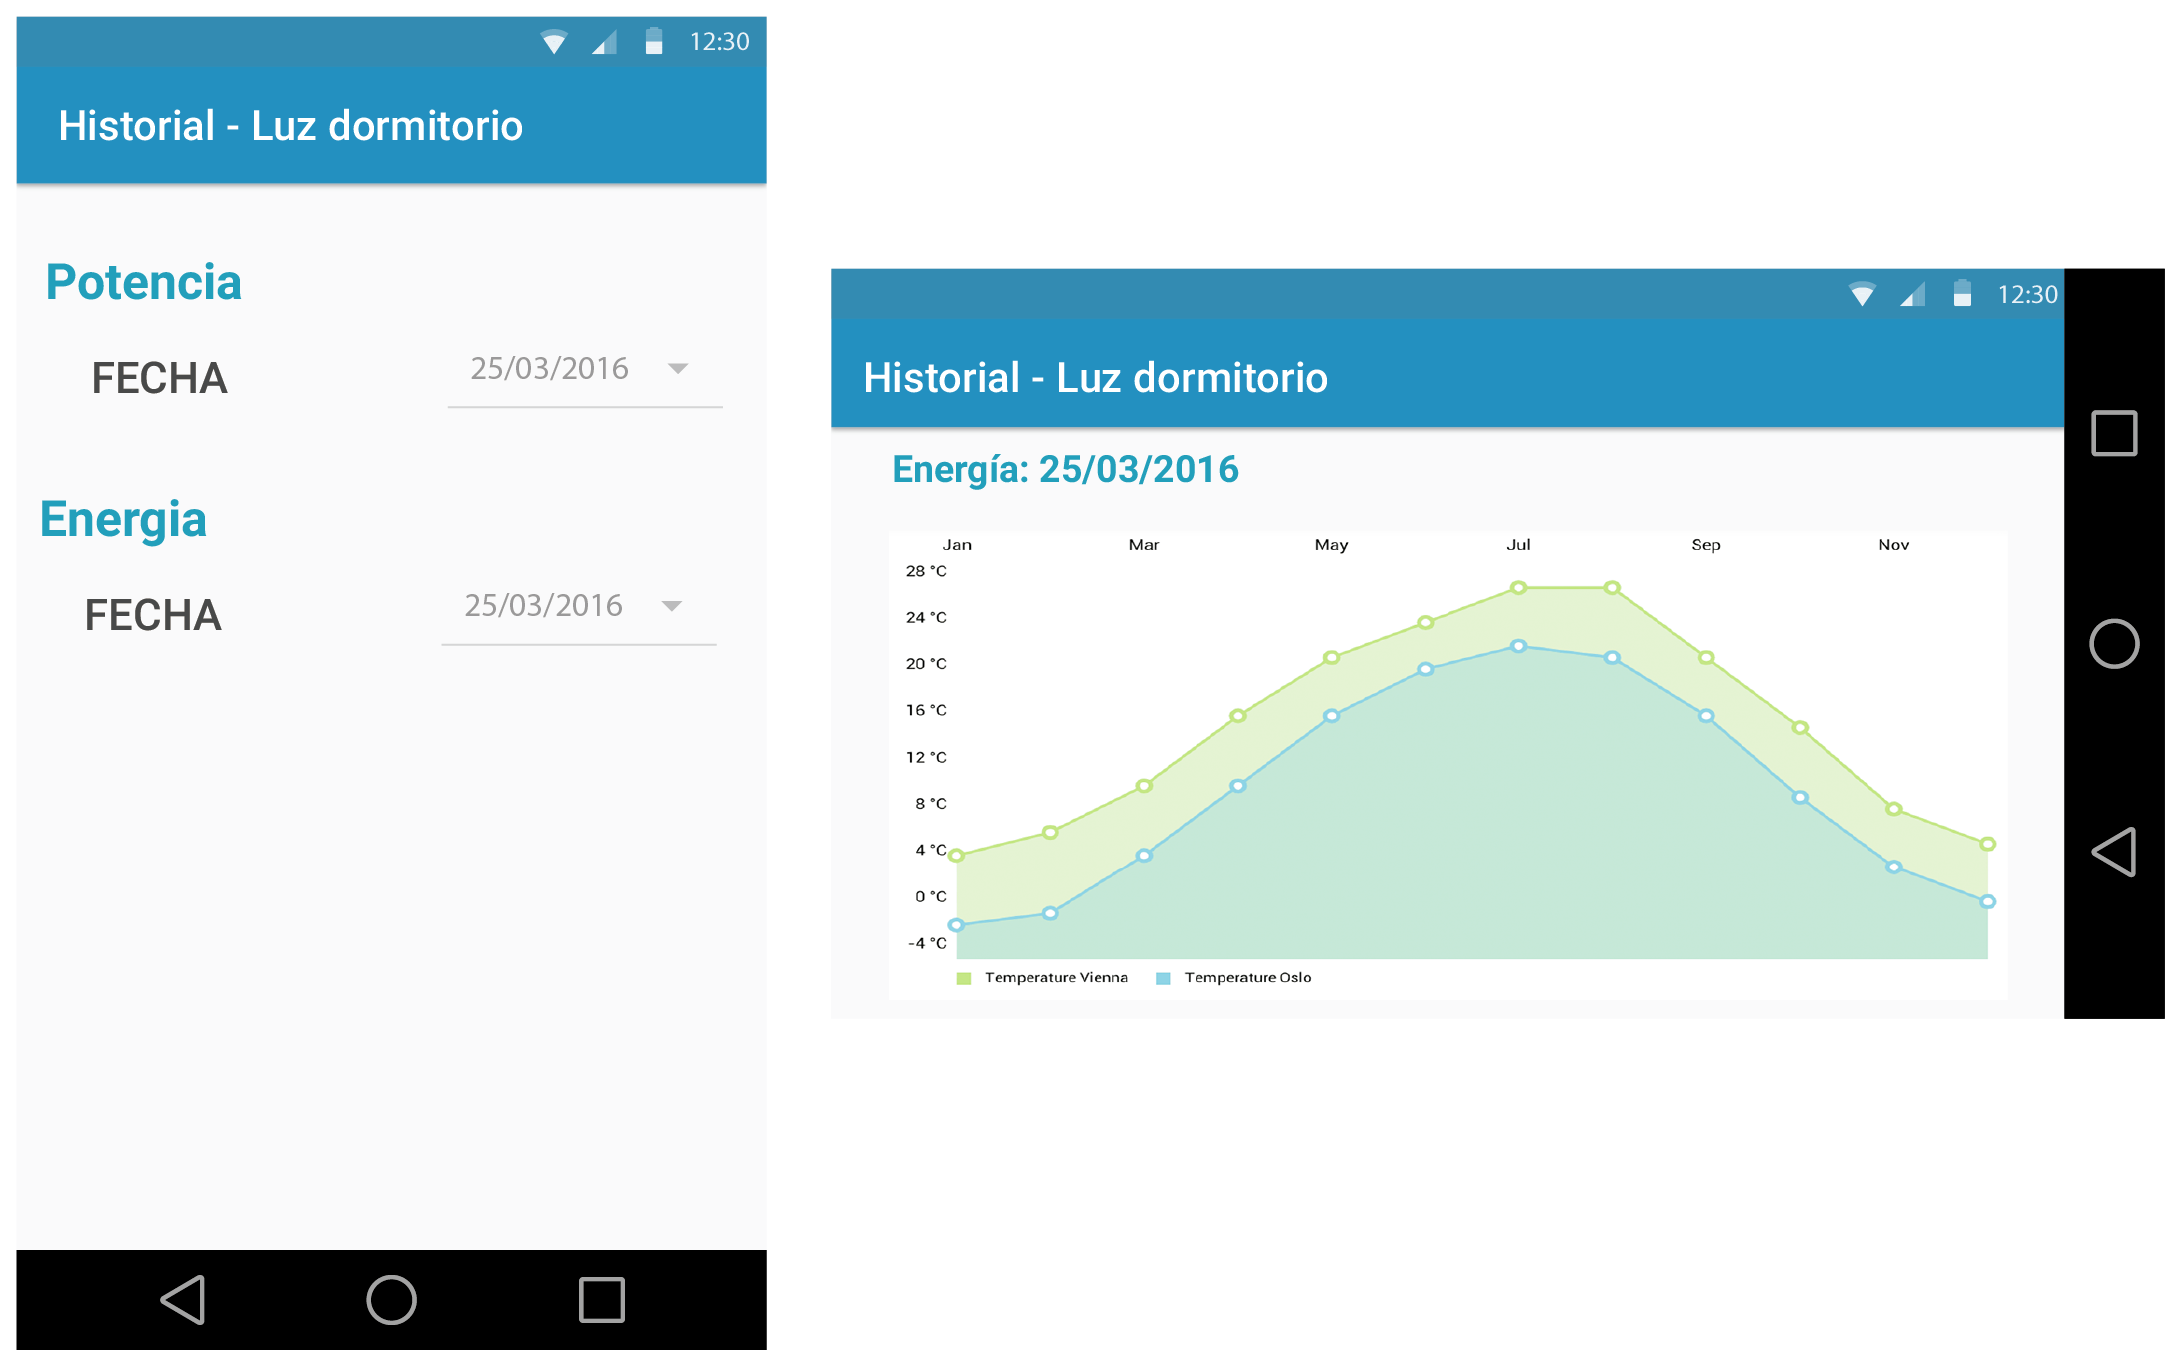
\includegraphics[width=14cm]{./Figures/3_3_1_app_wireframe_3.png}
	\caption{Detalle de la maqueta, pantallas 8 y 9.}
	\label{fig:app_wireframe_3}
\end{figure}


\item Pantalla 10 (parte izquierda de la Figura \ref{fig:app_wireframe_4}): contiene los parámetros configurables del Smart Plug seleccionado. Se accede a esta pantalla presionando la opción Configuración en el menú del botón de acción flotante. Los parámetros que se pueden configurar son básicamente tres: el nombre del dispositivo, el ícono del Smart Plug y la programación horaria para cada día de la semana.

En cuanto al nombre del dispositivo, se puede configurar un nombre de hasta 32 caracteres. Una vez ingresado se debe presionar la flecha que se encuentra a la derecha del control para ingresar el texto. Este nombre quedará configurado en el Smart Plug, por lo que todas las aplicaciones que tengan registrado a este Plug, verán el nuevo nombre.

Al presionar el ícono del Smart Plug se mostrará la pantalla 11 (parte central de la Figura \ref{fig:app_wireframe_4}), permitiendo elegir una imagen de una lista de íconos. Una vez que se selecciona uno de estos se vuelve a la pantalla 10. El ícono es una información propia de la aplicación móvil y no queda guardado en el Smart Plug. Por lo tanto, distintas aplicaciones móviles pueden asignar íconos diferentes a un mismo Plug.

Finalmente, la programación horaria puede ser habilitada y deshabilitada para cada día de la semana individualmente. La transparencia del recuadro que contiene la información de cada día indica si la programación horaria está habilitada: si el recuadro es semi-transparente, está deshabilitada, pero si no es transparente, está habilitada. 

Si se presiona cualquiera de los días se mostrará la pantalla 12 (parte derecha de la Figura \ref{fig:app_wireframe_4}) invitando a ingresar la hora de encendido de la carga. Se puede elegir cambiar esta hora o dejar la que estaba ya configurada. Una vez configurada la hora de encendido se volverá a mostrar la pantalla 12 para ingresar la hora de apagado; se procede de igual forma que antes. Cuando se ingresan ambas horas se configura el Smart Plug con estos nuevos valores.

Si en cambio de desea deshabilitar esta opción para un día de la semana, se debe mantener presionado el recuadro del día elegido. Cuando se deshabilite la opción, el recuadro se mostrará semi-transparente.

\end{itemize}


\begin{figure}[!h]
	\centering
	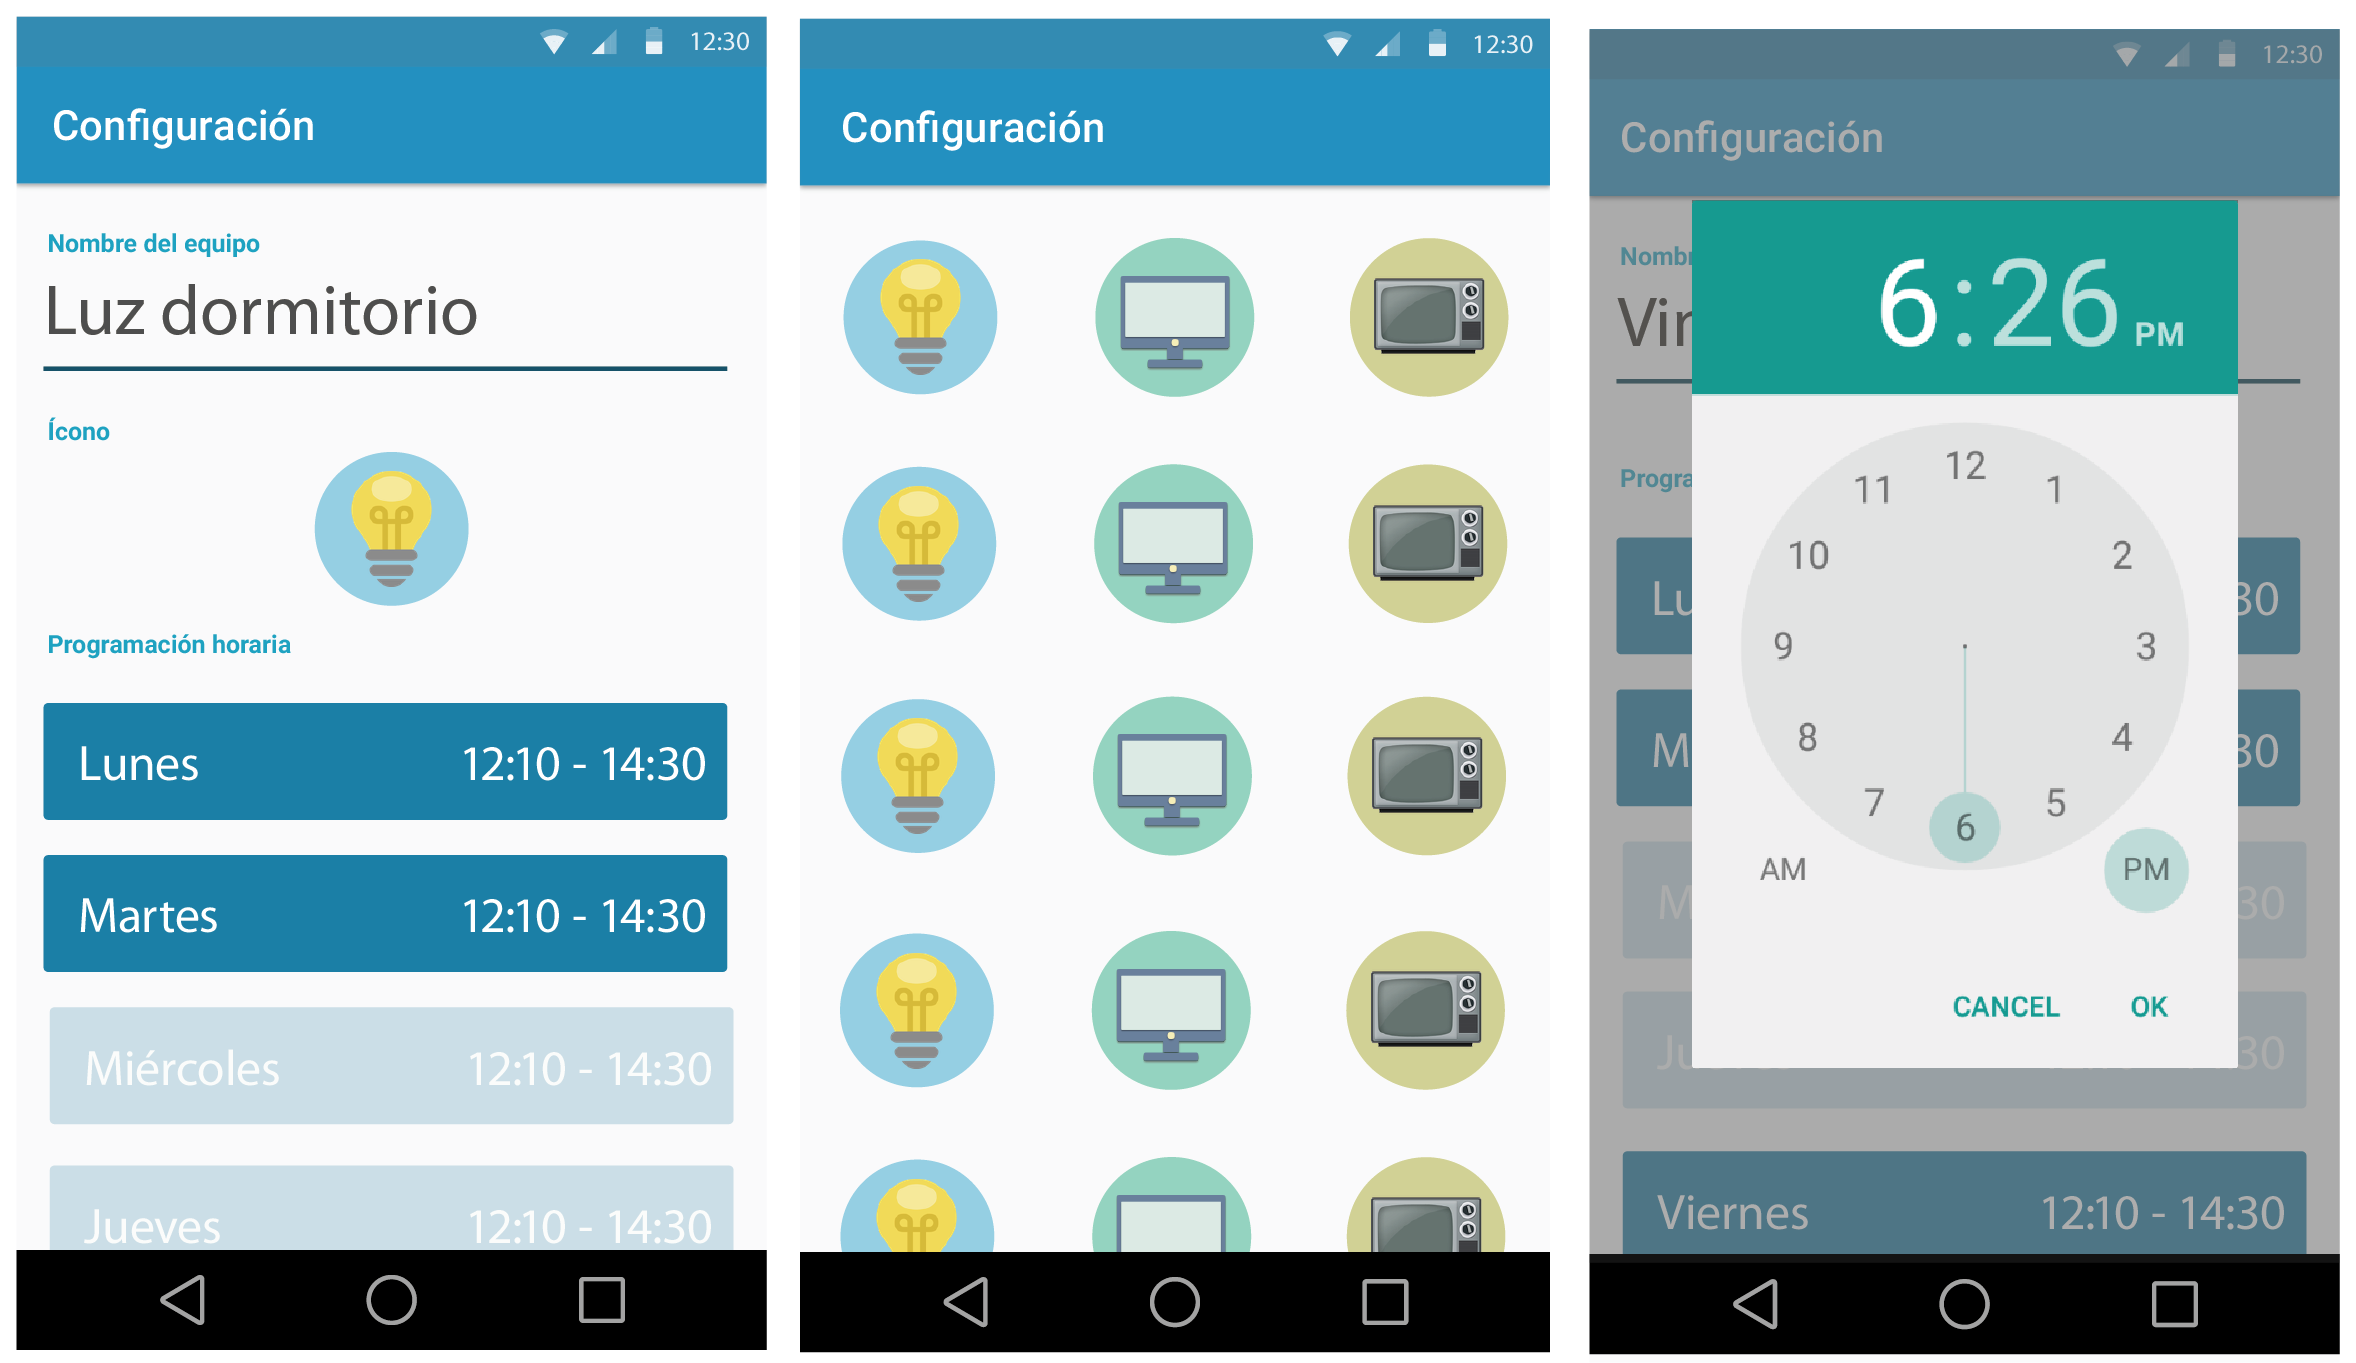
\includegraphics[width=14cm]{./Figures/3_3_1_app_wireframe_4.png}
	\caption{Detalle de la maqueta, pantallas 10, 11 y 12.}
	\label{fig:app_wireframe_4}
\end{figure}




\subsection{Arquitectura de la aplicación}
\label{subsec:arquitectura_app}

La estructura general de la aplicación móvil puede verse en la Figura \ref{fig:app_arquitectura}. A continuación se describirán los elementos principales que la componen y la interacción que existe entre ellos.

\begin{figure}[h]
	\centering
	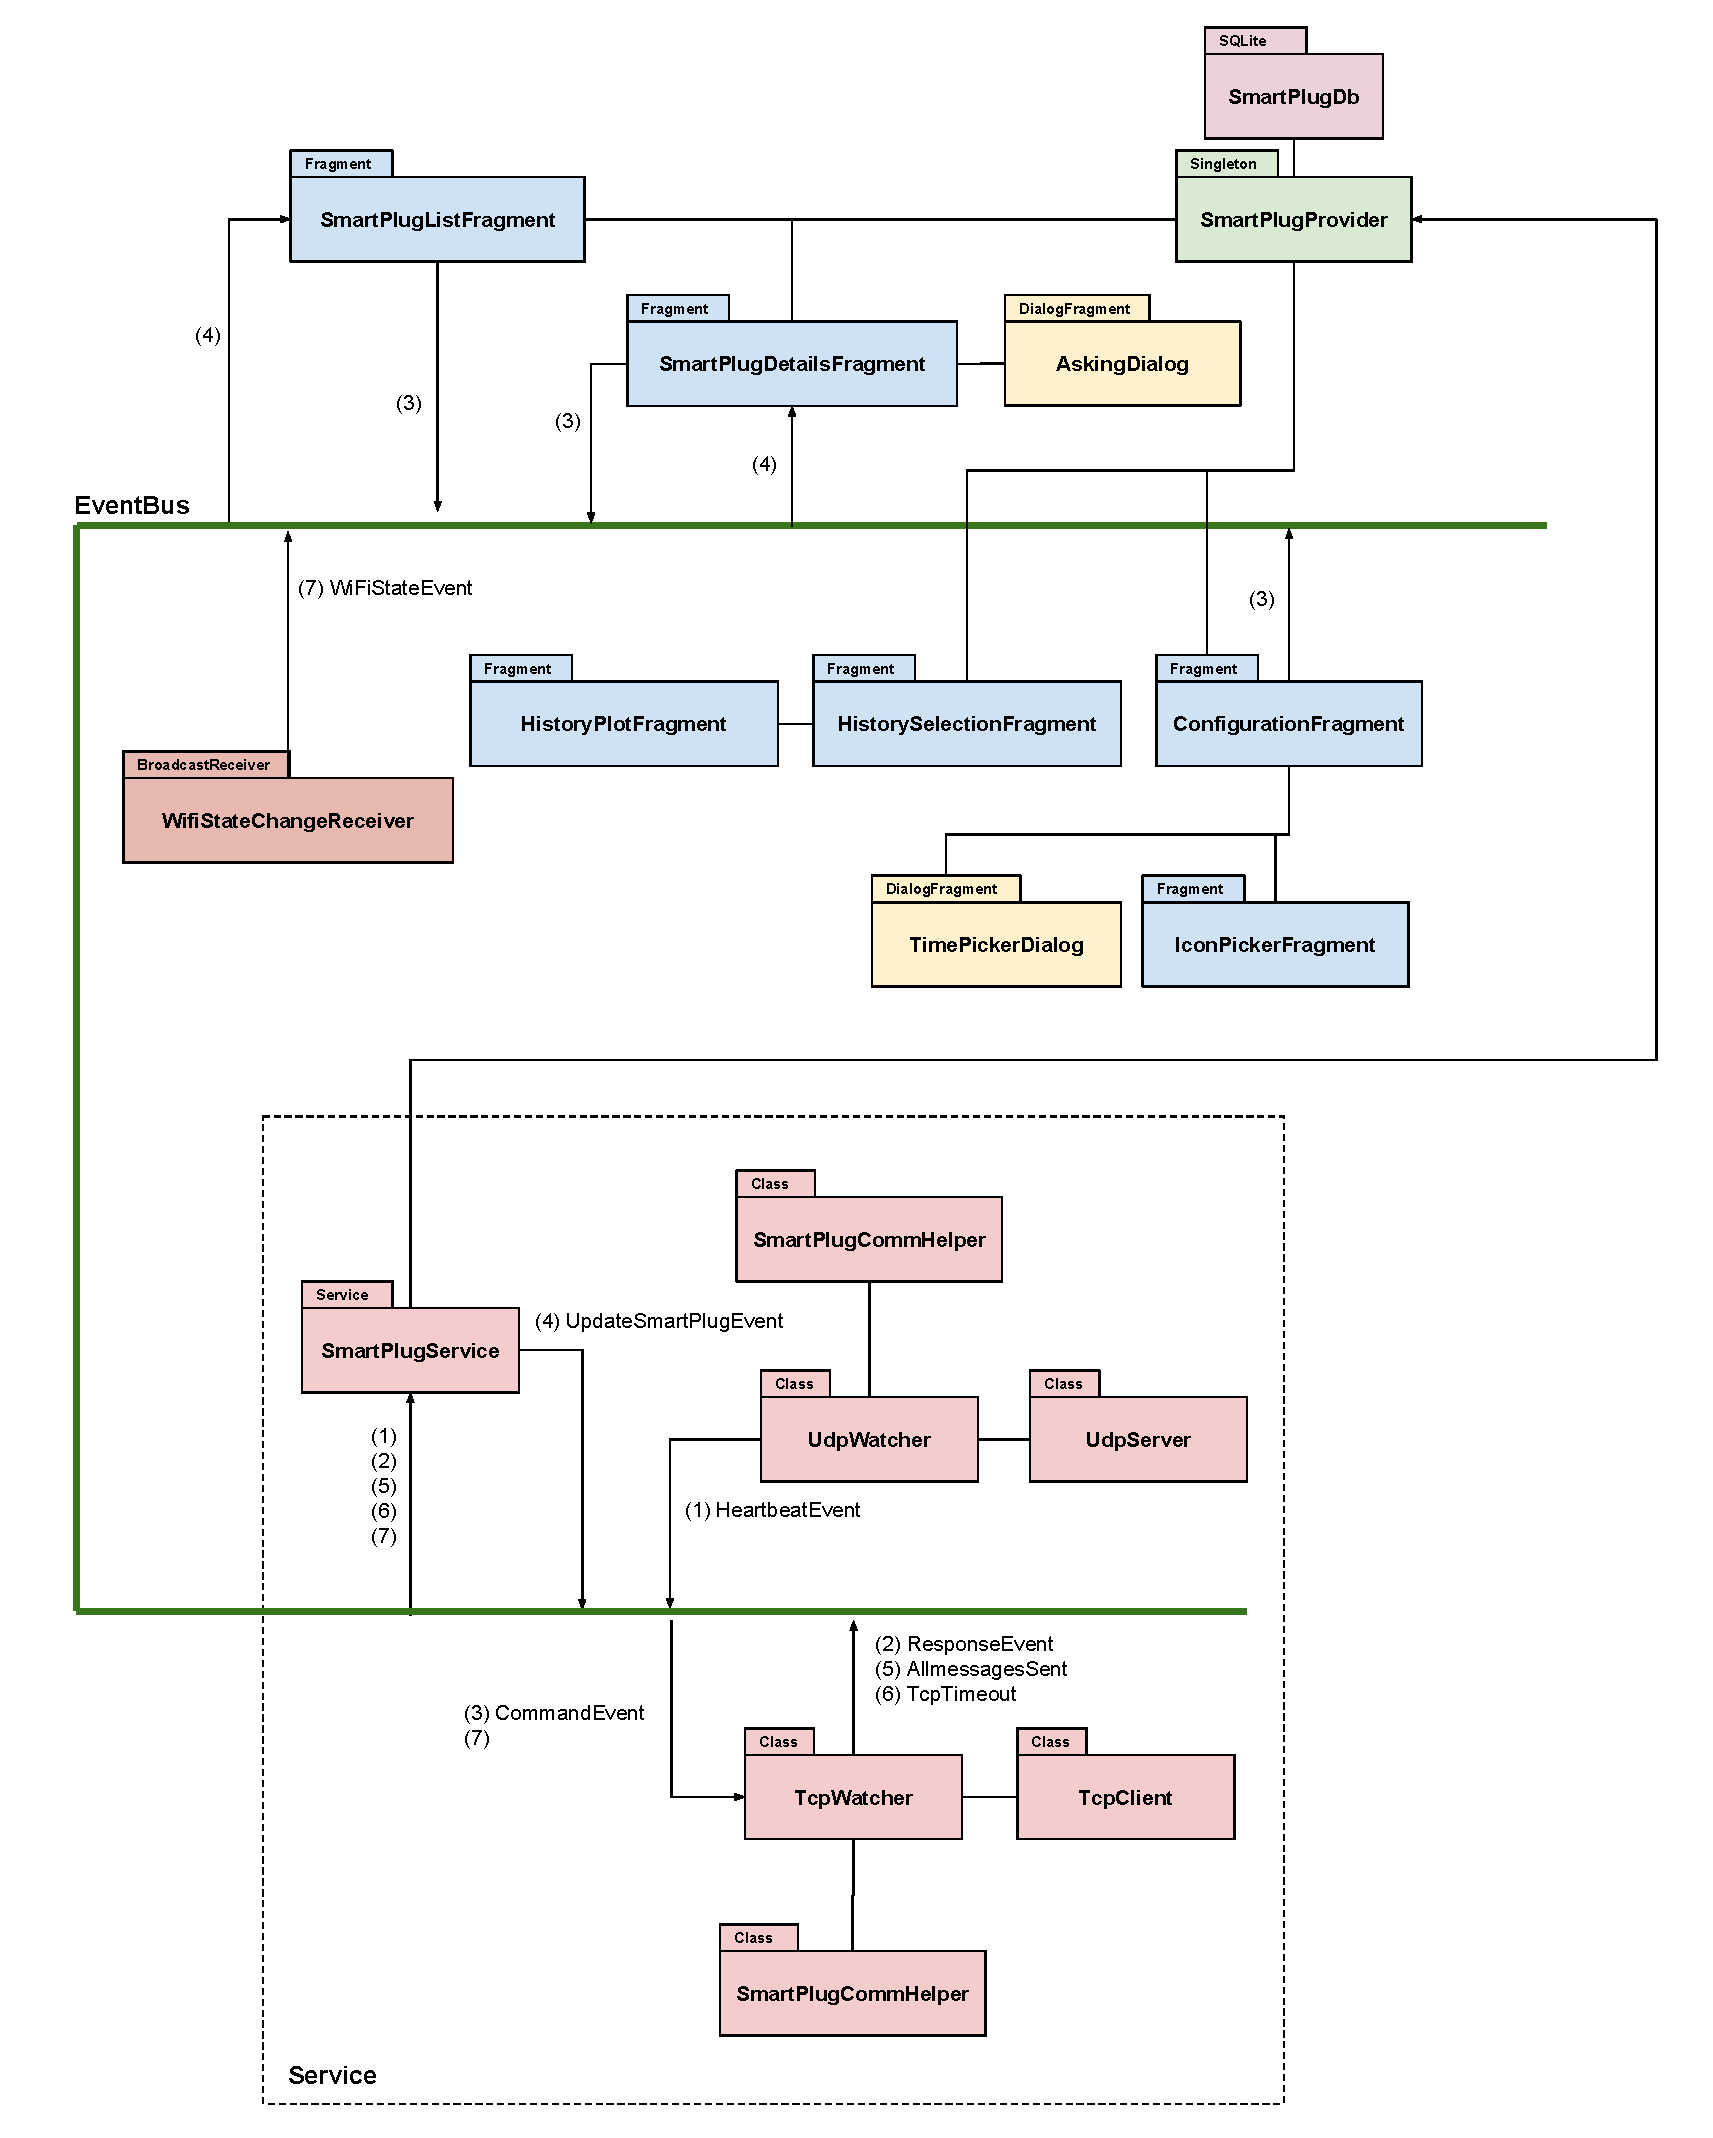
\includegraphics[width=14cm]{./Figures/3_3_2_app-arquitectura.pdf}
	\caption{Relación entre las clases desarrolladas para la aplicación móvil.}
	\label{fig:app_arquitectura}
\end{figure}

\begin{itemize}
\item EventBus. La forma que se eligió para comunicar todos los elementos de la aplicación es un bus de eventos. Para esto se utilizó una librería llamada EventBus, desarrollada por la empresa Green Robot \citep{eventbus_web}. Esta librería consiste en un esquema de suscripción a un bus en el que cualquier clase puede publicar un evento, el cual va a ser recibido por todas las clases que se hayan suscrito al mismo. Además, esta librería se encarga de la comunicación entre clases que se encuentran en distintos threads.

Los eventos no son más que objetos de java que contienen información de interés para la clase que los recibe. En el caso concreto de la aplicación, se crearon varios eventos, los cuales pueden verse en la Figura \ref{fig:app_arquitectura} representados mediante un número al lado de las flechas que unen las clases al bus de eventos común. Estos eventos son:


\begin{enumerate}
\item HeartbeatEvent: este evento se genera cada vez que el servidor UDP recibe un mensaje periódico de uno de los Smart Plugs. Con este mensaje se logra mantener actualizada la información del Smart Plug, especialmente la IP que le fue asignada por el DHCP dentro de la red WiFi.
\item ResponseEvent: contiene la respuesta recibida por el cliente TCP de la aplicación a un comando enviado a un Smart Plug.
\item CommandEvent: contiene los elementos de una trama que se tiene que enviar a un determinado Smart Plug. Cualquier componente de la aplicación que quiera enviar un mensaje a un Smart Plug debe enviar una instancia de este evento al EventBus.
\item UpdateSmartPlugEvent: este evento se genera cada vez que se recibe nueva información de un Smart Plug. De esta forma, los fragmentos que están suscritos a este evento actualizarán la información mostrada si el Smart Plug que se actualizó coincide con el que se está mostrando. 

Por ejemplo cuando se enciende la carga de un Smart Plug desde la lista de Plugs, este evento permite que la transparencia del ícono del Plug cambie al recibir la confirmación de que la carga fue encendida. Si no estuviera este evento el ícono se actualizaría cuando se regenerara la vista del fragmento.
\item AllmessagesSent: se genera cuando el cliente TCP de la aplicación no tiene más mensajes que enviar. Se utiliza para que la aplicación libere ciertos recursos que retiene mientras se están enviando los mensajes.
\item TcpTimeout: se genera cuando se produce un timeout esperando la respuesta a un comando, o cuando se produce otro error en la comunicación. Cada uno de estos errores y timeouts se van sumando en un contador asociado a cada Smart Plug y cuando se superan los 5 eventos, se indica que existe un problema en la comunicación con el Plug.
\item WiFiStateEvent: se genera cada vez que cambia el estado de la conexión del teléfono a la red WiFi. Esto le sirve a la aplicación para conocer si está conectado a la red WiFi o no. En caso de no estarlo, no se intentan enviar mensajes a los Plugs ya que no se los va a poder alcanzar.
\end{enumerate}

\item Servicio. Cuando se inicia la aplicación por primera vez, esta inicia una instancia de la clase SmartPlugService que hereda a la clase Service de Android. Un servicio permite implementar una parte de la lógica que se debe ejecutar por un tiempo prolongado en un thread distinto del thread principal de la aplicación. Además, como fue configurado en el caso de esta aplicación, este servicio se mantiene ejecutándose aún cuando la aplicación se encuentra cerrada.

Dentro del servicio se implementa la lógica para la consulta periódica de los Smart Plugs que identificó la aplicación. Cada 10 minutos, el servicio se ejecutará y realizará una serie de consultas a todos los Smart Plugs que conozca, preguntando el último valor de las mediciones, algunos parámetros de configuración para ver si fueron cambiados por otra aplicación y el estado de la carga, para ver si fue conmutada por otra aplicación.

Además, cada 1 hora aproximadamente, el servicio le pedirá a todos los Smart Plugs las mediciones históricas del día para conocer los valores de potencia activa y energía consumida de la última hora.

Toda la información que es recibida desde los Smart Plugs es volcada a una base de datos propia de la aplicación (smartPlug.db) la cual va a ser consultada por todos los otros elementos de la aplicación cuando necesiten conocer la última información de un Smart Plug. El acceso a la base de datos se realiza a través de la clase SmartPlugProvider.

La ejecución periódica de este servicio se logra configurando una alarma mediante el AlarmManager de Android. Esta alarma se dispara cada 10 minutos. A las 6 veces que se ejecute esta alarma, se considerará que pasó una hora y se harán las consultas correspondientes a los Plugs.


\item TcpWatcher y TcpClient. Estas clases se ocupan de establecer la comunicación TCP con los distintos Smart Plugs. La clase TcpWatcher se suscribe a los eventos de tipo CommandEvent y cada vez que recibe uno lo coloca dentro de una lista, la cual va a ir siendo leída para determinar las tramas que debe enviar. La comunicación propiamente dicha está implementada en la clase TcpClient, la cual gestiona la conexión y los posibles errores que se pueden producir. 

Para armar las tramas de acuerdo a lo establecido por el protocolo desarrollado en este trabajo, la clase TcpWatcher utiliza los métodos de la clase SmartPlugCommHelper que se encarga de encapsular los formatos de las tramas de acuerdo al comando y registro que se está manipulando.

Si se recibe una respuesta del Smart Plug, la clase TcpWatcher generará un evento del tipo ResponseEvent. En caso de que se produzca un error, generará un evento del tipo TcpTimeout. Cuando termine de enviar todos los mensajes que tenía pendientes generará el mensaje AllmessagesSent.

\item UdpWatcher y UdpServer. Este par de clases se ocupa de escuchar los mensajes periódicos que son enviados a la dirección de \textit{broadcast} de la red por parte de los Smart Plugs. Los mensajes periódicos son enviados al puerto UDP 55555. Cada vez que UdpServer (que es la clase que implementa concretamente el servidor UDP) recibe un nuevo datagrama UDP, se lo comunica a la clase UdpWatcher.

La clase UdpWatcher parsea el datagrama con la ayuda de la clase SmartPlugCommHelper y determina de qué Smart Plug provino. Con esta información genera un evento del tipo HeartbeatEvent. Dentro del datagrama UDP se encuentra el ID único que identifica a cada Smart Plug, el cual se va a utilizar dentro de la aplicación para identificar unívocamente a un Plug.

\item SmartPlugProvider. Es la clase encargada de acceder a la base de datos de la aplicación (smartPlug.db) en donde está contenida la información de los Smart Plugs encontrados. Esta base de datos está compuesta por 4 tablas, las cuales pueden verse en la Figura \ref{fig:app_sqlite}. A continuación se da una breve descripción de cada tabla:

\begin{itemize}
\item StaticInfo. Contiene la información básica del Smart Plug: su nombre y el ícono que tiene asociado. Todas las entradas de las tablas van a estar asociadas al número de ID único del Smart Plug el cual es recibido en cada mensaje UDP que envía el Plug.
\item OnOffTimes. Contiene los horarios de encendido y apagado para cada día de la semana así como también una variable que indica qué días están habilitados.
\item Measurements. Contiene las mediciones históricas recibidas desde cada Smart Plug. En cada entrada de la tabla se guarda la fecha a la que corresponden las mediciones y las 24 mediciones de ese día, al igual que el tipo de medición (potencia activa o energía consumida).
\item InstantaneousInfo. Contiene información variable de cada Smart Plug. Es información incluye: la última IP en la que se encontró al Smart Plug, la última fecha y hora de comunicación, el estado de la carga, las últimas mediciones instantáneas, la cantidad de timeouts que se produjeron en la comunicación y el estado de la comunicación.
\end{itemize}

Toda clase que desee acceder a la base de datos, debe hacerlo a través de la clase SmartPlugProvider ya que implementa toda la lógica relacionada con la manipulación de la base de datos.

\item WiFiStateChangeReceiver. Es una clase que extiende a BroadcastReceiver y se encarga de recibir los intents de Android relacionados con los cambios en la conectividad. De esta forma determina si el teléfono se encuentra conectado a la red WiFi o no. En caso de no estar conectado los mensajes a los Smart Plugs no se envían.

\end{itemize}


\begin{figure}[h]
	\centering
	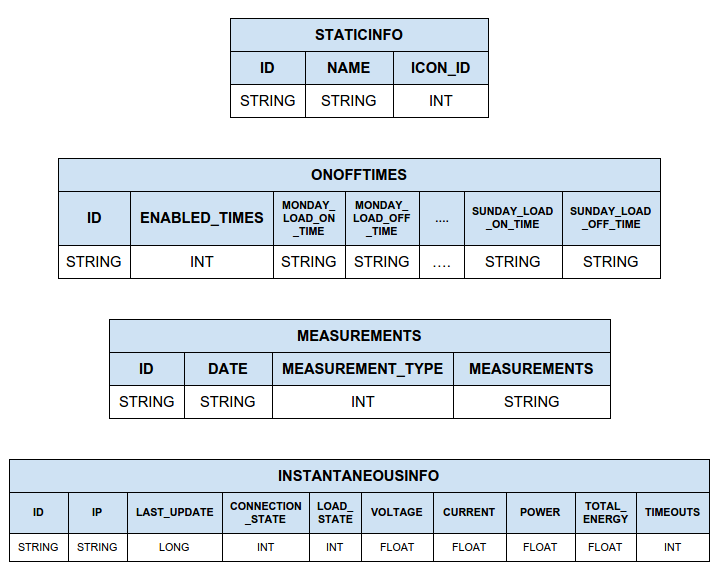
\includegraphics[width=13cm]{./Figures/3_3_2_tablas_sqlite.png}
	\caption{Tablas que componen la base de datos de la aplicación.}
	\label{fig:app_sqlite}
\end{figure}

La lógica asociada a cada una de las pantallas mostradas en la maqueta en la Subsección \ref{subsec:app_wireframe} se implementaron mediante fragments, para flexibilizar el diseño de la interfaz gráfica. La relación entre las pantallas de la Figura \ref{fig:app_wireframe} y los nombres de los fragmentos es la siguiente:

\begin{enumerate}
\item Pantalla 1: SplashScreenFragment.
\item Pantalla 2: SmartPlugListFragment.
\item Pantalla 3: SmartPlugDetailsFragment.
\item Pantalla 4: SmartPlugDetailsFragment.
\item Pantalla 5: AskingDialog.
\item Pantalla 6: AskingDialog.
\item Pantalla 7: AskingDialog.
\item Pantalla 8: HistorySelectionFragment.
\item Pantalla 9: HistoryPlotFragment.
\item Pantalla 10: ConfigurationFragment.
\item Pantalla 11: IconPickerFragment.
\item Pantalla 12: TimePickerDialog.
\end{enumerate}

La lógica de alto nivel que implementa cada fragment fue explicada en la Subsección \ref{subsec:app_wireframe}. El código fuente de la aplicación puede encontrarse en \citep{repo_app}.

